%  LaTeX support: latex@mdpi.com 
%  For support, please attach all files needed for compiling as well as the log file, and specify your operating system, LaTeX version, and LaTeX editor.

%=================================================================
\documentclass[hardware,article,submit,pdftex,moreauthors]{Definitions/mdpi} 

%--------------------
% Class Options:
%--------------------
%----------
% journal
%----------
% Choose between the following MDPI journals:
% acoustics, actuators, addictions, admsci, adolescents, aerobiology, aerospace, agriculture, agriengineering, agrochemicals, agronomy, ai, air, algorithms, allergies, alloys, analytica, analytics, anatomia, animals, antibiotics, antibodies, antioxidants, applbiosci, appliedchem, appliedmath, applmech, applmicrobiol, applnano, applsci, aquacj, architecture, arm, arthropoda, arts, asc, asi, astronomy, atmosphere, atoms, audiolres, automation, axioms, bacteria, batteries, bdcc, behavsci, beverages, biochem, bioengineering, biologics, biology, biomass, biomechanics, biomed, biomedicines, biomedinformatics, biomimetics, biomolecules, biophysica, biosensors, biotech, birds, bloods, blsf, brainsci, breath, buildings, businesses, cancers, carbon, cardiogenetics, catalysts, cells, ceramics, challenges, chemengineering, chemistry, chemosensors, chemproc, children, chips, cimb, civileng, cleantechnol, climate, clinpract, clockssleep, cmd, coasts, coatings, colloids, colorants, commodities, compounds, computation, computers, condensedmatter, conservation, constrmater, cosmetics, covid, crops, cryptography, crystals, csmf, ctn, curroncol, cyber, dairy, data, ddc, dentistry, dermato, dermatopathology, designs, devices, diabetology, diagnostics, dietetics, digital, disabilities, diseases, diversity, dna, drones, dynamics, earth, ebj, ecologies, econometrics, economies, education, ejihpe, electricity, electrochem, electronicmat, electronics, encyclopedia, endocrines, energies, eng, engproc, entomology, entropy, environments, environsciproc, epidemiologia, epigenomes, est, fermentation, fibers, fintech, fire, fishes, fluids, foods, forecasting, forensicsci, forests, foundations, fractalfract, fuels, future, futureinternet, futurepharmacol, futurephys, futuretransp, galaxies, games, gases, gastroent, gastrointestdisord, gels, genealogy, genes, geographies, geohazards, geomatics, geosciences, geotechnics, geriatrics, grasses, gucdd, hazardousmatters, healthcare, hearts, hemato, hematolrep, heritage, higheredu, highthroughput, histories, horticulturae, hospitals, humanities, humans, hydrobiology, hydrogen, hydrology, hygiene, idr, ijerph, ijfs, ijgi, ijms, ijns, ijpb, ijtm, ijtpp, ime, immuno, informatics, information, infrastructures, inorganics, insects, instruments, inventions, iot, j, jal, jcdd, jcm, jcp, jcs, jcto, jdb, jeta, jfb, jfmk, jimaging, jintelligence, jlpea, jmmp, jmp, jmse, jne, jnt, jof, joitmc, jor, journalmedia, jox, jpm, jrfm, jsan, jtaer, jvd, jzbg, kidneydial, kinasesphosphatases, knowledge, land, languages, laws, life, liquids, literature, livers, logics, logistics, lubricants, lymphatics, machines, macromol, magnetism, magnetochemistry, make, marinedrugs, materials, materproc, mathematics, mca, measurements, medicina, medicines, medsci, membranes, merits, metabolites, metals, meteorology, methane, metrology, micro, microarrays, microbiolres, micromachines, microorganisms, microplastics, minerals, mining, modelling, molbank, molecules, mps, msf, mti, muscles, nanoenergyadv, nanomanufacturing,\gdef\@continuouspages{yes}} nanomaterials, ncrna, ndt, network, neuroglia, neurolint, neurosci, nitrogen, notspecified, %%nri, nursrep, nutraceuticals, nutrients, obesities, oceans, ohbm, onco, %oncopathology, optics, oral, organics, organoids, osteology, oxygen, parasites, parasitologia, particles, pathogens, pathophysiology, pediatrrep, pharmaceuticals, pharmaceutics, pharmacoepidemiology,\gdef\@ISSN{2813-0618}\gdef\@continuous pharmacy, philosophies, photochem, photonics, phycology, physchem, physics, physiologia, plants, plasma, platforms, pollutants, polymers, polysaccharides, poultry, powders, preprints, proceedings, processes, prosthesis, proteomes, psf, psych, psychiatryint, psychoactives, publications, quantumrep, quaternary, qubs, radiation, reactions, receptors, recycling, regeneration, religions, remotesensing, reports, reprodmed, resources, rheumato, risks, robotics, ruminants, safety, sci, scipharm, sclerosis, seeds, sensors, separations, sexes, signals, sinusitis, skins, smartcities, sna, societies, socsci, software, soilsystems, solar, solids, spectroscj, sports, standards, stats, std, stresses, surfaces, surgeries, suschem, sustainability, symmetry, synbio, systems, targets, taxonomy, technologies, telecom, test, textiles, thalassrep, thermo, tomography, tourismhosp, toxics, toxins, transplantology, transportation, traumacare, traumas, tropicalmed, universe, urbansci, uro, vaccines, vehicles, venereology, vetsci, vibration, virtualworlds, viruses, vision, waste, water, wem, wevj, wind, women, world, youth, zoonoticdis 
% For posting an early version of this manuscript as a preprint, you may use "preprints" as the journal. Changing "submit" to "accept" before posting will remove line numbers.

%---------
% article
%---------
% The default type of manuscript is "article", but can be replaced by: 
% abstract, addendum, article, book, bookreview, briefreport, casereport, comment, commentary, communication, conferenceproceedings, correction, conferencereport, entry, expressionofconcern, extendedabstract, datadescriptor, editorial, essay, erratum, hypothesis, interestingimage, obituary, opinion, projectreport, reply, retraction, review, perspective, protocol, shortnote, studyprotocol, systematicreview, supfile, technicalnote, viewpoint, guidelines, registeredreport, tutorial
% supfile = supplementary materials

%----------
% submit
%----------
% The class option "submit" will be changed to "accept" by the Editorial Office when the paper is accepted. This will only make changes to the frontpage (e.g., the logo of the journal will get visible), the headings, and the copyright information. Also, line numbering will be removed. Journal info and pagination for accepted papers will also be assigned by the Editorial Office.

%------------------
% moreauthors
%------------------
% If there is only one author the class option oneauthor should be used. Otherwise use the class option moreauthors.

%---------
% pdftex
%---------
% The option pdftex is for use with pdfLaTeX. Remove "pdftex" for (1) compiling with LaTeX & dvi2pdf (if eps figures are used) or for (2) compiling with XeLaTeX.

%=================================================================
% MDPI internal commands - do not modify
\firstpage{1} 
\makeatletter 
\setcounter{page}{\@firstpage} 
\makeatother
\pubvolume{1}
\issuenum{1}
\articlenumber{0}
\pubyear{2024}
\copyrightyear{2024}
%\externaleditor{Academic Editor: Firstname Lastname}
\datereceived{ } 
\daterevised{ } % Comment out if no revised date
\dateaccepted{ } 
\datepublished{ } 
%\datecorrected{} % For corrected papers: "Corrected: XXX" date in the original paper.
%\dateretracted{} % For corrected papers: "Retracted: XXX" date in the original paper.
\hreflink{https://doi.org/} % If needed use \linebreak
%\doinum{}
%\pdfoutput=1 % Uncommented for upload to arXiv.org
%\CorrStatement{yes}  % For updates


%=================================================================
% Add packages and commands here. The following packages are loaded in our class file: fontenc, inputenc, calc, indentfirst, fancyhdr, graphicx, epstopdf, lastpage, ifthen, float, amsmath, amssymb, lineno, setspace, enumitem, mathpazo, booktabs, titlesec, etoolbox, tabto, xcolor, colortbl, soul, multirow, microtype, tikz, totcount, changepage, attrib, upgreek, array, tabularx, pbox, ragged2e, tocloft, marginnote, marginfix, enotez, amsthm, natbib, hyperref, cleveref, scrextend, url, geometry, newfloat, caption, draftwatermark, seqsplit
% cleveref: load \crefname definitions after \begin{document}

\usepackage{datatool}
\usepackage{longtable}
\usepackage{booktabs}
\usepackage{pdflscape}

%=================================================================
% Please use the following mathematics environments: Theorem, Lemma, Corollary, Proposition, Characterization, Property, Problem, Example, ExamplesandDefinitions, Hypothesis, Remark, Definition, Notation, Assumption
%% For proofs, please use the proof environment (the amsthm package is loaded by the MDPI class).

%=================================================================
% Full title of the paper (Capitalized)
\Title{A portable wave tank and wave energy converter for engineering dissemination and outreach}

% MDPI internal command: Title for citation in the left column
\TitleCitation{A portable wave tank and wave energy converter for engineering dissemination and outreach}


\newcommand{\orcidauthorA}{0000-0003-0738-3772} % Ryan
\newcommand{\orcidauthorB}{0009-0002-5318-9225} % Gerrit
\newcommand{\orcidauthorC}{0000-0002-1208-2352} % Giorgio
\newcommand{\orcidauthorD}{0000-0001-8994-7257} % Dominic
\newcommand{\orcidauthorE}{0000-0002-1732-5261} % Steve


% \newcommand{\orcidauthorGiorgio}{XX}
% \newcommand{\orcidauthorDominic}{XX}

% Authors, for the paper (add full first names)
\Author{Nicholas Ross$^{1,\ddagger}$, Delaney Heileman$^{1,\ddagger}$, A. Gerrit Motes$^{1,\ddagger}$\orcidB{}, Anwi Fomukong$^{1,\ddagger}$, Giorgio Bacelli$^{1,\ddagger}$\orcidC{}, Steven~J.~Spencer$^{1,\ddagger}$\orcidE{}, Dominic D. Forbush$^{1,\ddagger}$\orcidD{}, Kevin Dullea$^{1,\ddagger}$ and Ryan G. Coe$^{1,\ddagger}$\orcidA{}*}

% Author Orchid ID: enter ID or remove command

% %\newcommand{\orcidauthorB}{0000-0000-0000-000X} % Add \orcidB{} behind the author's name

% % Authors, for the paper (add full first names)
% \Author{Firstname Lastname $^{1,\dagger,\ddagger}$\orcidA{}, Firstname Lastname $^{2,\ddagger}$ and Firstname Lastname $^{2,}$*}

%\longauthorlist{yes}

% MDPI internal command: Authors, for metadata in PDF
\AuthorNames{Nicholas Ross, Delaney Heileman, A. Gerrit Motes, Anwi Fomukong, Giorgio Bacelli, Steven~J.~Spencer, Dominic D. Forbush, Kevin Dullea and Ryan G. Coe}

% MDPI internal command: Authors, for citation in the left column
\AuthorCitation{Ross, N. et al.}
% If this is a Chicago style journal: Lastname, Firstname, Firstname Lastname, and Firstname Lastname.

% Affiliations / Addresses (Add [1] after \address if there is only one affiliation.)
\address{%
$^{1}$ \quad Sandia National Laboratories}
% $^{2}$ \quad Affiliation 2; e-mail@e-mail.com}

% Contact information of the corresponding author
\corres{Correspondence: rcoe@sandia.gov}

% Current address and/or shared authorship
\firstnote{Current address: Affiliation.}  % Current address should not be the same as any items in the Affiliation section.
\secondnote{These authors contributed equally to this work.}
% The commands \thirdnote{} till \eighthnote{} are available for further notes

%\simplesumm{} % Simple summary

%\conference{} % An extended version of a conference paper

% Abstract (Do not insert blank lines, i.e. \\) 
\abstract{
Wave energy converters are a nascent energy generation technology that harness the power in ocean waves.
To assist in communicating both fundamental and complex concepts of wave energy, a small scale portable wave tank and wave energy converter have been developed.
The system has been designed using commercial off-the-shelf components and all design hardware and software are openly available for replication.
Accompanying educational curriculum has also been developed to assist in using this hardware for classroom education.
}

% Keywords
\keyword{wave energy; educational; outreach} 

% The fields PACS, MSC, and JEL may be left empty or commented out if not applicable
%\PACS{J0101}
%\MSC{}
%\JEL{}

%%%%%%%%%%%%%%%%%%%%%%%%%%%%%%%%%%%%%%%%%%
% Only for the journal Diversity
%\LSID{\url{http://}}

%%%%%%%%%%%%%%%%%%%%%%%%%%%%%%%%%%%%%%%%%%
% Only for the journal Applied Sciences
%\featuredapplication{Authors are encouraged to provide a concise description of the specific application or a potential application of the work. This section is not mandatory.}
%%%%%%%%%%%%%%%%%%%%%%%%%%%%%%%%%%%%%%%%%%

%%%%%%%%%%%%%%%%%%%%%%%%%%%%%%%%%%%%%%%%%%
% Only for the journal Data
%\dataset{DOI number or link to the deposited data set if the data set is published separately. If the data set shall be published as a supplement to this paper, this field will be filled by the journal editors. In this case, please submit the data set as a supplement.}
%\datasetlicense{License under which the data set is made available (CC0, CC-BY, CC-BY-SA, CC-BY-NC, etc.)}

%%%%%%%%%%%%%%%%%%%%%%%%%%%%%%%%%%%%%%%%%%
% Only for the journal Toxins
%\keycontribution{The breakthroughs or highlights of the manuscript. Authors can write one or two sentences to describe the most important part of the paper.}

%%%%%%%%%%%%%%%%%%%%%%%%%%%%%%%%%%%%%%%%%%
% Only for the journal Encyclopedia
%\encyclopediadef{For entry manuscripts only: please provide a brief overview of the entry title instead of an abstract.}

%%%%%%%%%%%%%%%%%%%%%%%%%%%%%%%%%%%%%%%%%%
% Only for the journal Advances in Respiratory Medicine and Smart Cities
%\addhighlights{yes}
%\renewcommand{\addhighlights}{%

%\noindent This is an obligatory section in “Advances in Respiratory Medicine'' and ``Smart Cities”, whose goal is to increase the discoverability and readability of the article via search engines and other scholars. Highlights should not be a copy of the abstract, but a simple text allowing the reader to quickly and simplified find out what the article is about and what can be cited from it. Each of these parts should be devoted up to 2~bullet points.\vspace{3pt}\\
%\textbf{What are the main findings?}
% \begin{itemize}[labelsep=2.5mm,topsep=-3pt]
% \item First bullet.
% \item Second bullet.
% \end{itemize}\vspace{3pt}
%\textbf{What is the implication of the main finding?}
% \begin{itemize}[labelsep=2.5mm,topsep=-3pt]
% \item First bullet.
% \item Second bullet.
% \end{itemize}
%}

%%%%%%%%%%%%%%%%%%%%%%%%%%%%%%%%%%%%%%%%%%
\begin{document}

%%%%%%%%%%%%%%%%%%%%%%%%%%%%%%%%%%%%%%%%%%
\section{Introduction}
The Sandia Interactive Wave Energy Education Display (SIWEED) is a small scale wave tank and wave energy converter (WEC) that is designed to be portable and serve in outreach and dissemination of wave energy research.
The development of this system was inspired by previous research at Sandia National Laboratories in the areas of WEC device and control design and testing.
Specifically, the SIWEED demonstrates the causal feedback control and device design principles described in \citet{Bacelli2020} and \citet{Coe2020a}.


A wide variety of similar educational wave tanks and tow tanks have been built, but few have been documented.
\citet{unger2006creating} reworked a tow tank at MIT to enable remote operation via the internet.
A tank with a similar scale ($\sim$2\,m) and focus was developed by \cite{Trust2015}, but oriented at demonstrating the effectiveness of coastal flood controls.
There seem to have been two major iterations, one electrically driven by a paddle like wave maker, and one plunger type driven mechanically by hand. 
That team has also made multiple similar hydraulic flume tanks for demonstration purposes.
An educational wave tank in currently on display at the National Museum of Scotland, but the waves do not interact with any bodies on the surface \cite{Ivan2016}. 
%\citet{Y.H.Yu} Made a wave tank to study floating- point absorbers as wave energy converters, showing similarities to this project, but they use a flap-type wavemaker, and their tank is much larger and not portable.

SIWEED is a novel expansion on similar small-scale educational wave tanks, as the wave maker is driven by a ball screw, and the user is able to control both the waves and the WEC device.
The parameters of the wave are also fully controllable with a number of operational modes (see Table~\ref{tab:wave_maker_controls}).
The sea state mode outputs a JONSWAP spectrum \cite{Hasselmann1973} to imitate a natural wave environment with random waves\footnote{Note that pseudo-random phasing is used.}.
Initially, the primary intended audience for SIWEED was college students and above, but there now exists curriculum in the design files for lower age groups, and the GUI can be toggled to run a simplified version.

\begin{table}[tb]
  \caption{Wave maker function modes and control parameters.}
  \label{tab:wave_maker_controls}
  \centering

  \begin{tabular}{rl}
  \hline
  \textbf{Control mode}      & \textbf{Input parameters}        \\
  \hline
  Jog                        & Position, $z$ {[}mm{]}                \\
  \hline
  \multirow{2}{*}{Function}  & Amplitude, $A$ {[}mm{]}               \\
                             & Frequency, $f$ {[}Hz{]}               \\
  \hline
  \multirow{3}{*}{Sea state} & Significant wave height, $H_s$ {[}mm{]} \\
                             & Peak frequency, $f_p$ {[}Hz{]}          \\
                             & Peakedness, $\gamma$ {[} {]}               \\       
  \hline
  \end{tabular}
\end{table}


\section{Design} % Describe the hardware, highlighting the customization rather than the steps of the procedure. Highlight how it differs/which advantage it offers over pre-existing methods. For example, how could this hardware: be compared to other hardware in terms of cost or ease of use, be used in the development of further designs in a particular area, and so on. Add 3-5 bulleted points to broadly explain to other researchers how the hardware could be potentially useful to them, for either standard or novel laboratory tasks, inside or outside of the original user community.
The SIWEED is composed of a 1.5\,m $\times{}$ 0.3\,m $\times{}$ 0.5\,m acrylic tank, filled to roughly 0.3\,m deep, housing a vertical plunger style wave maker (see, e.g., \cite{hyun1976simplified}), and a single body WEC modeled on the WaveBot~\cite{Coe2016a}.
This tank size was chosen based to satisfy the competing objectives of keeping the tank small enough to allow for transportation while making the tank large enough to improve repeatability and performance.
Attached to the tank is a scale model of an ocean side town, meant to represent a potential power load.
The town is equipped with four lighting zones, which allow the simulated power output to be physically represented.
A CAD rendering of the system is shown in \figurename~\ref{fig:CAD} and a photograph is shown in \figurename~\ref{fig:siweed_photo_with_callouts}.
The system is centrally controlled by a Windows PC running a graphical user interface (GUI) developed using Processing\footnote{\url{https://processing.org}} and the controlP5 library\footnote{\url{http://www.sojamo.de/libraries/controlP5/}}.
Separate hardware nodes are then manages by two Arduinos.

\begin{figure}[tb]
  \centering
  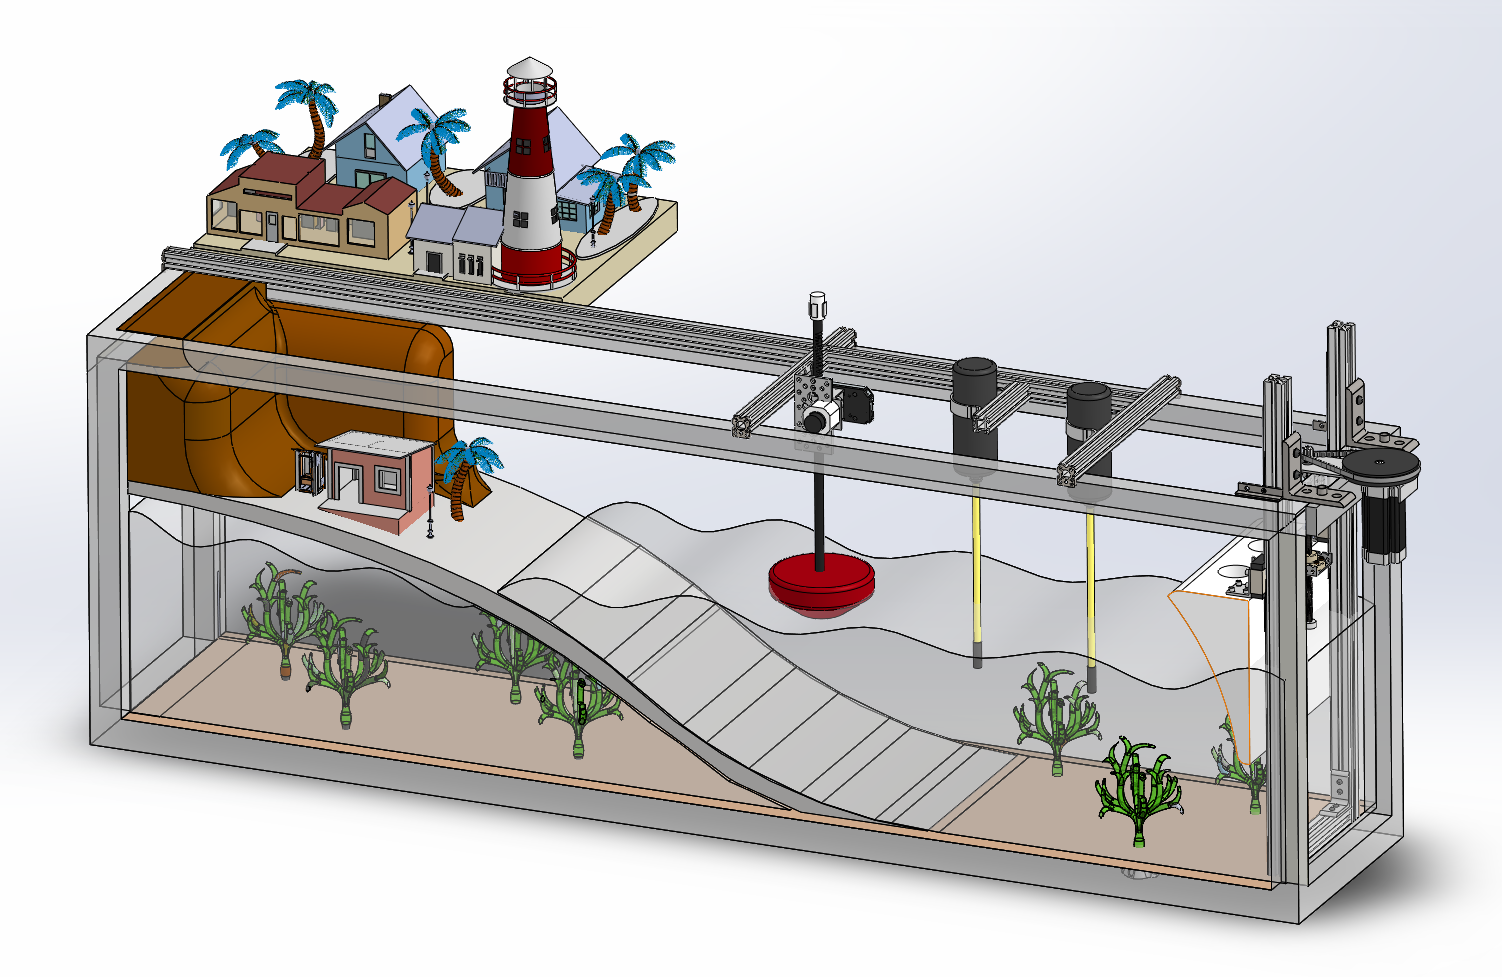
\includegraphics[width=1\textwidth]{diagrams/SIWEED_CAD.png}
  \caption{SIWEED CAD assembly rendering.}
  \label{fig:CAD}
\end{figure}

\begin{figure}[tb]
  \centering
  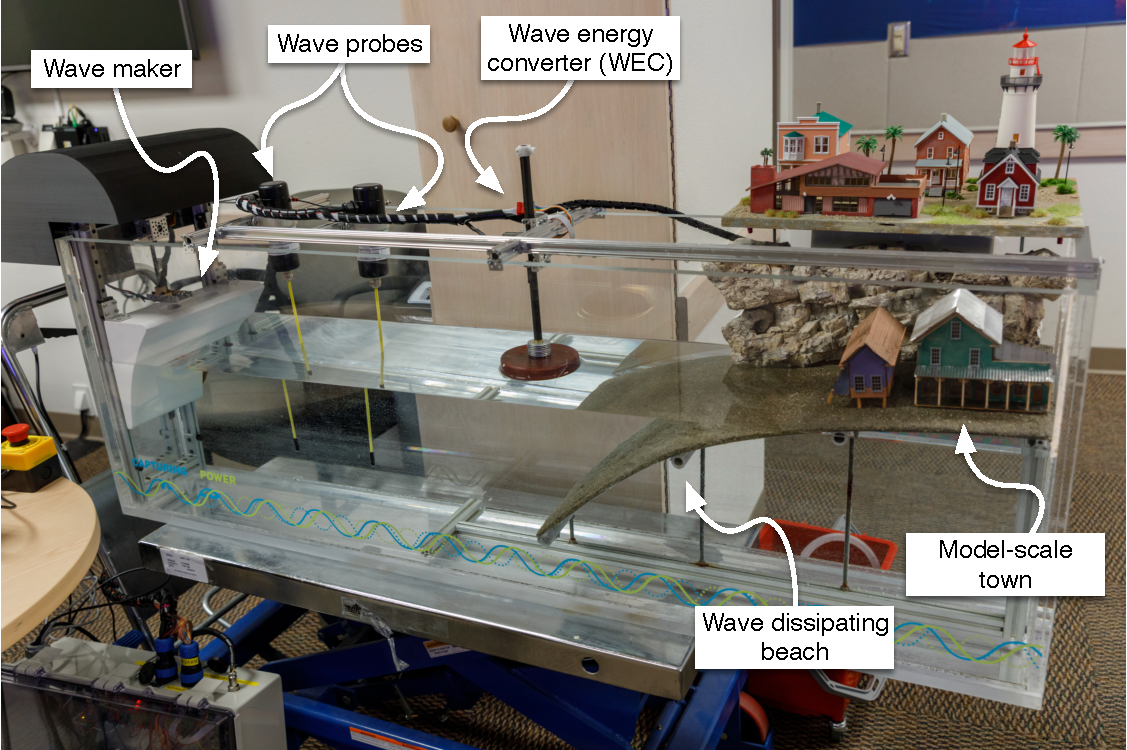
\includegraphics[width=1\textwidth]{diagrams/siweed_photo_with_callouts.pdf}
  \caption{Photograph of SIWEED system showing key system elements.}
  \label{fig:siweed_photo_with_callouts}
\end{figure}

\subsection{Hardware}
A system diagram for the SIWEED is shown in \figurename~\ref{fig:siweed_layout}.
Two Arduino Due micro controllers are used to control and acquire signals from the WEC and wave maker, communicating with the GUI through USB serial.
The Windows laptop acts as the core of the system, with the two Arduino Dues attached through USB. 
Each Arduino is then attached to the various devices it communicates with.
It is worth noting that Arduino Due model was selected for their higher clock speeds, but since they operate at 3.3\,V, multiple level shifters are used to enable communication between the Arduino Dues and the components that use 5\,V logic (see \figurename~\ref{fig:siweed_layout}).

The Windows laptop runs a Processing application that acts as the GUI, data logger, and serial communication manager.
The Arduinos receive their commands from Processing over USB serial, and perform individual control loops based on control states dictated by the GUI.
One Due controls the movement of the wave maker plunger, while the other controls the torque feedback of the WEC and lights in the model town.
Each send data back to the Processing GUI for data logging and plotting purposes.
The Arduino Dues each have a number of components they communicate with through various protocols (PWM, SPI, Analog).
These perform tasks like encoder buffering, motor control, and signal generation.
The connections can be seen in \figurename~\ref{fig:siweed_layout}.

\subsection{Graphical User Interface}
The SIWEED GUI is intended to be used with a touchscreen interface, but it is also fully functional with a mouse/track pad.
A screen shot of the GUI is shown in \figurename~\ref{fig:siweed_guiScreenShot}.
It is divided into three sections: The left instructional side, ``Mission Control", and ``System Status".

\begin{figure}[tb]
  \centering
  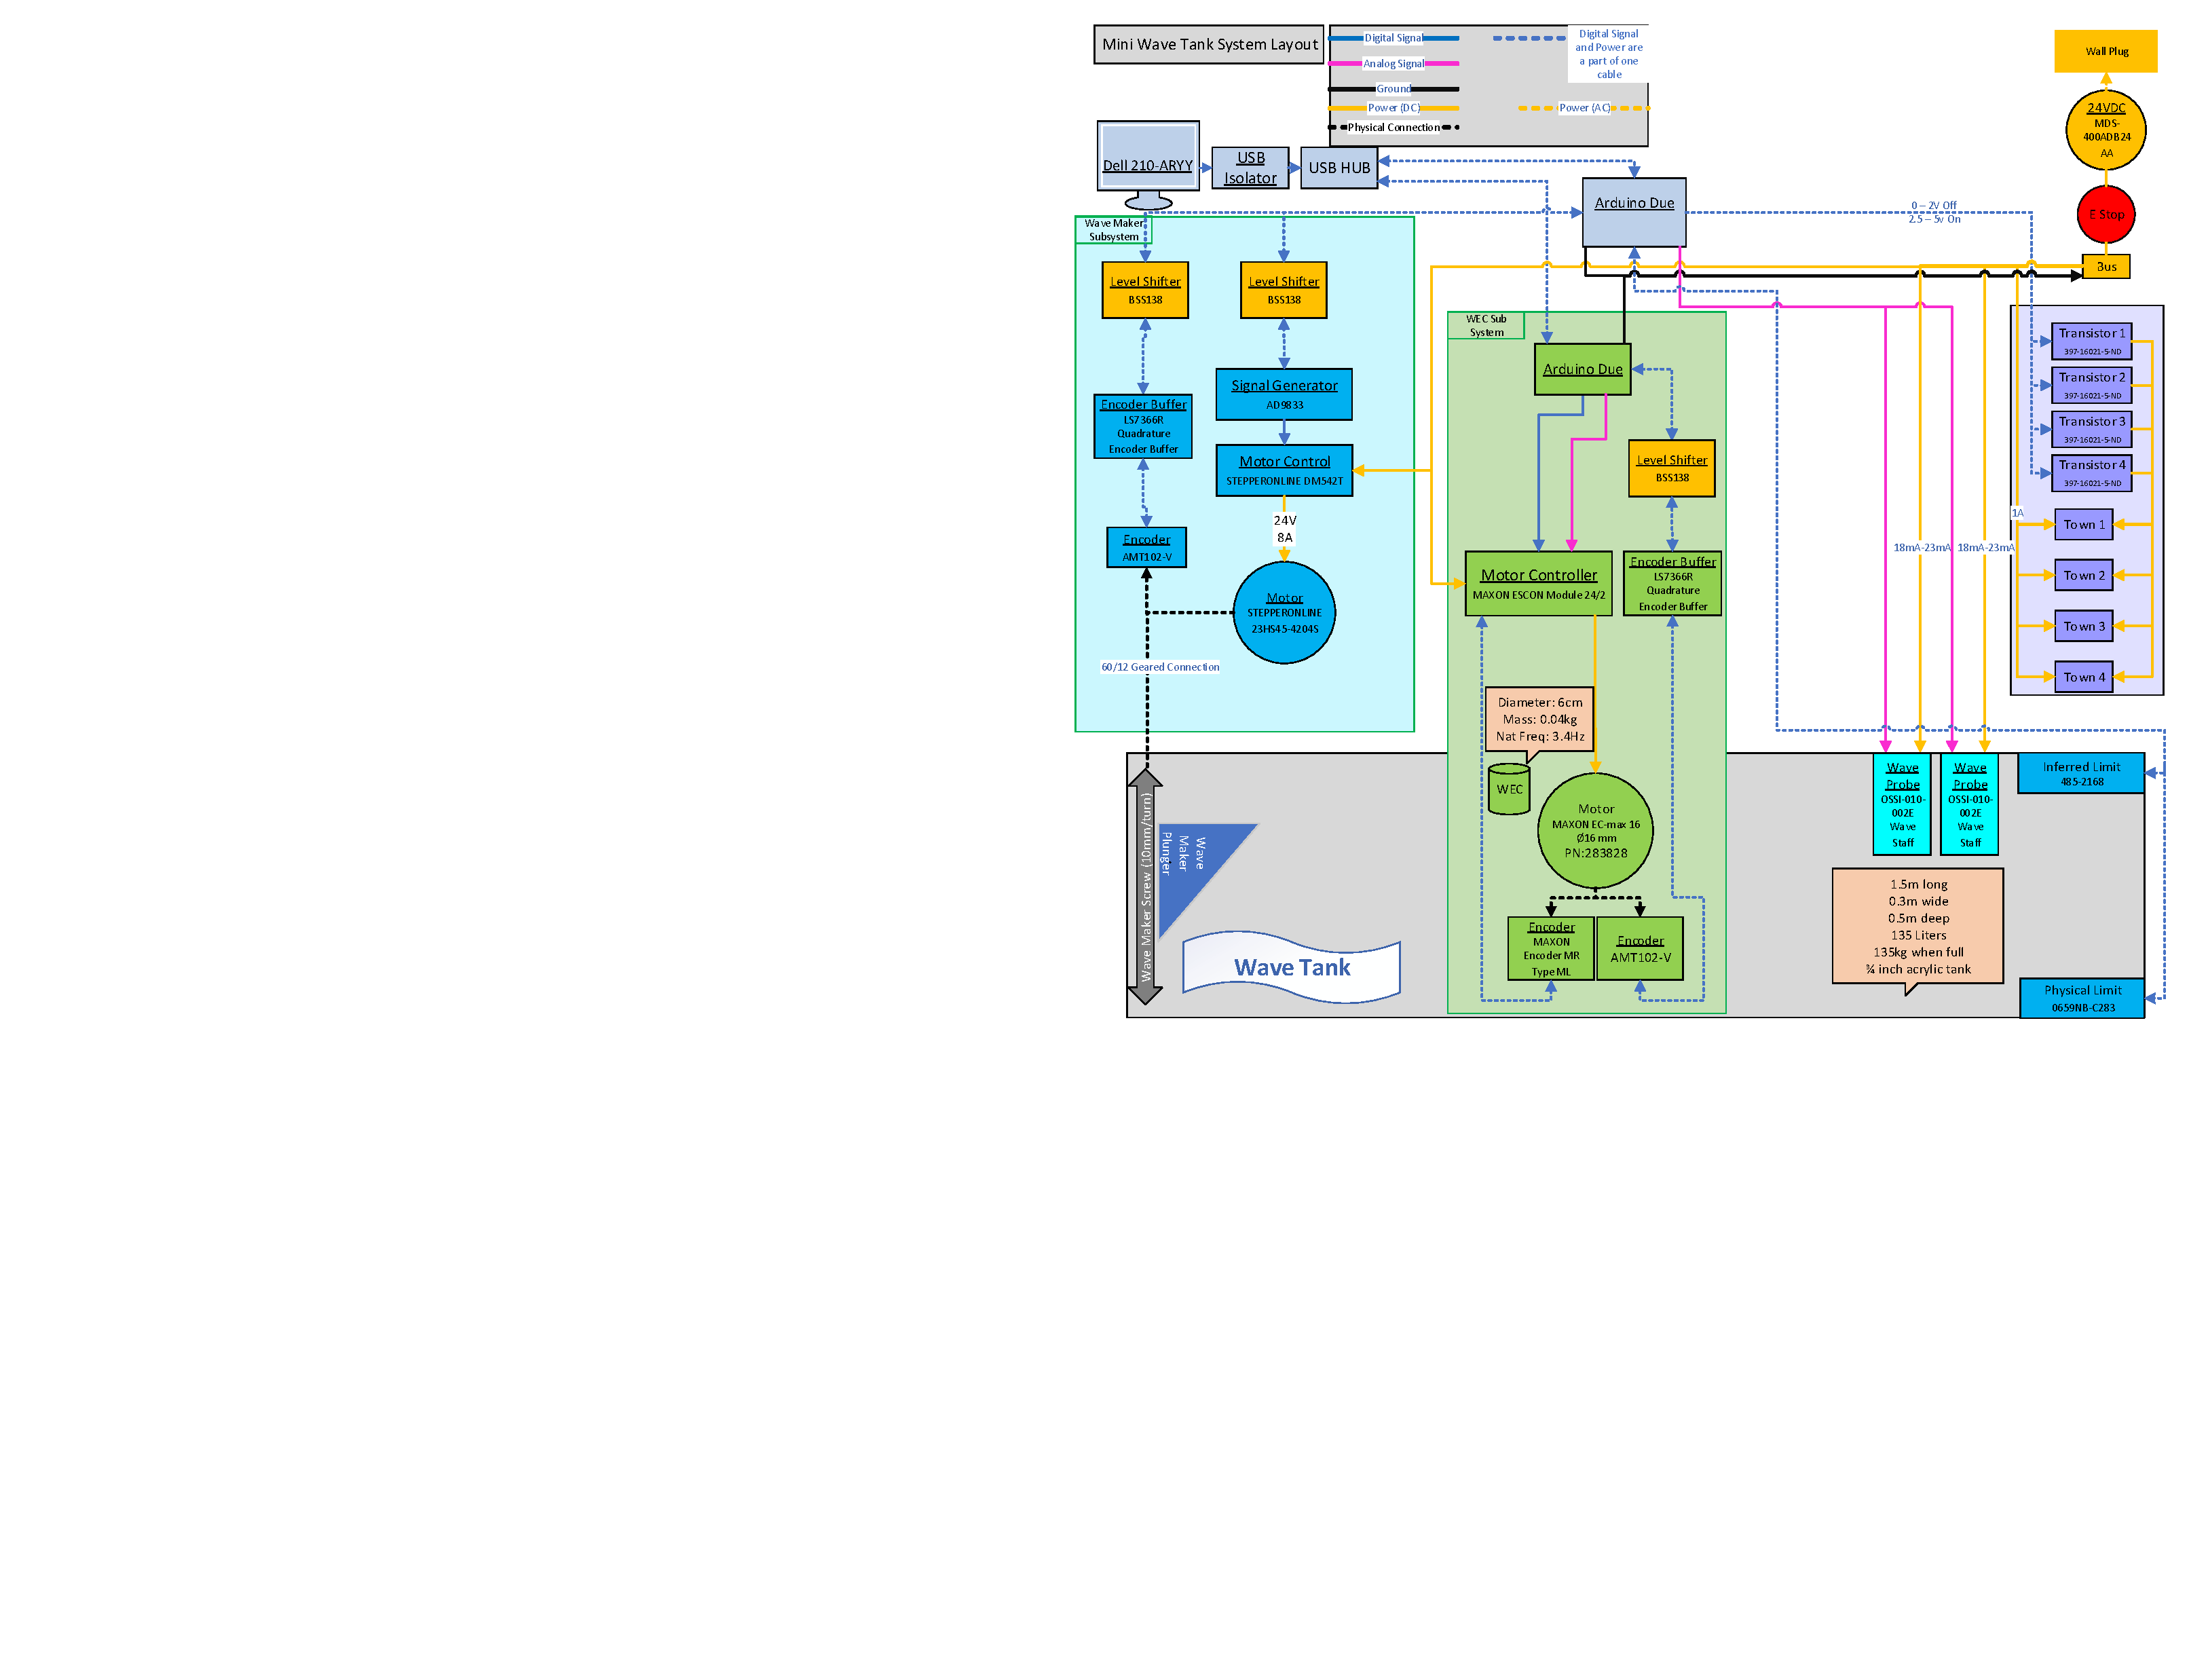
\includegraphics[width=1\textwidth]{diagrams/SystemLayout.pdf}
  \caption{SIWEED system layout diagram.}
  \label{fig:siweed_layout}
\end{figure}

\begin{figure}[tb]
  \centering
  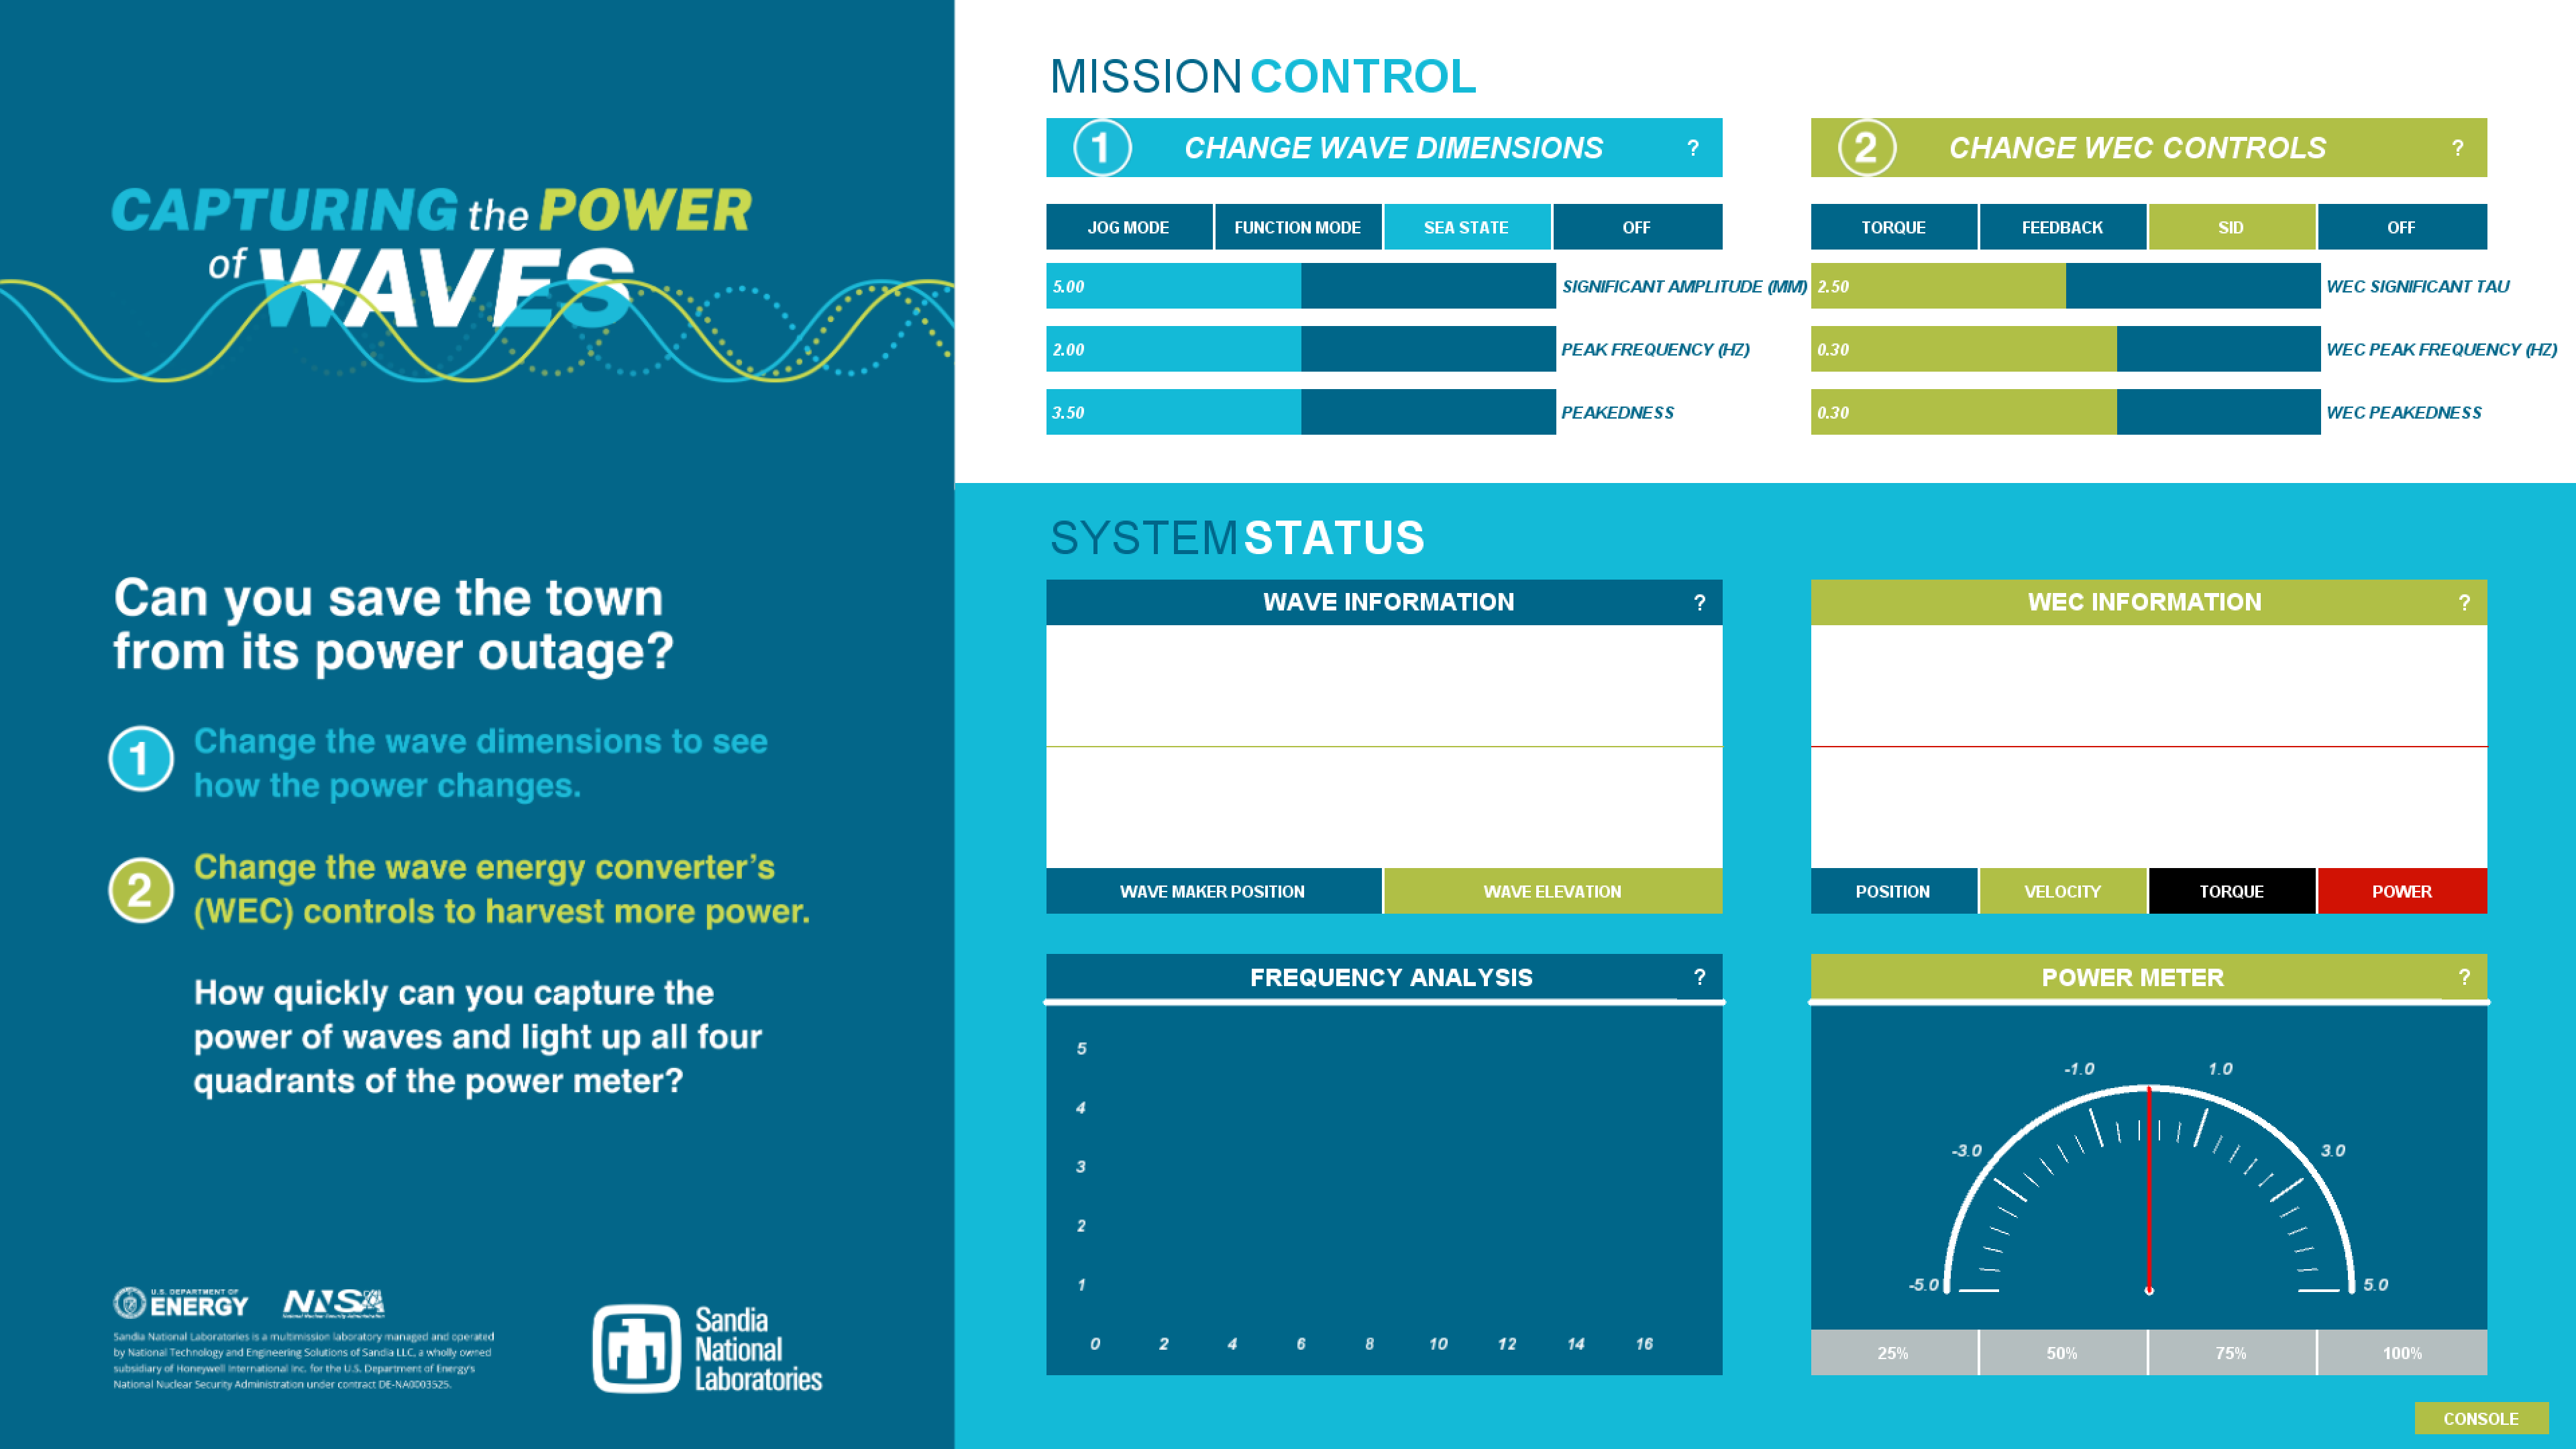
\includegraphics[width=1\textwidth]{diagrams/siweed_guiScreenShot.png}
  \caption{Graphical user interface (GUI) screenshot.}
  \label{fig:siweed_guiScreenShot}
\end{figure}

The left side of the ``Mission Control" section of the GUI pertains to control of the wave maker, which allows the user to switch between operational modes (``jog,'' ``function,'' ``sea state,'' and ``off'') and set the relevant parameters.
If, for example, the system is in ``sea state'' mode, the user can set the significant wave height ($H_s$), peak frequency ($f_p$), and peakedness factor ($\gamma$) for a JONSWAP wave spectrum.
The ``function" mode commands a simple sine wave, and so the parameters are amplitude and frequency. 
The ``jog" mode simply commands a static position for the plunger to go to, so the only input parameter is that command position.
There are only as many input sliders displayed as there are inputs to the active control mode. 
For example, if the selected mode was ``jog", only one slider would be present in that section of the GUI for the user to interact with.

The right side of the ``Mission Control" section of the GUI contains controls for the WEC, which can be set into ``torque'' mode; in which the user directly sets a commanded torque, ``feedback'' mode; where proportional and integral feedback factors can be set by the user; ``SID'' mode, for system identification, allowing for open-loop multi-sine signals to be set by the user; and ``off.''
The ``SID'' mode works with the same inputs and JONSWAP control method as the ``Sea State'' mode for the wave maker, but commanding torque instead of position.
Where the purpose of the JONSWAP in the wave maker controls is to replicate a natural wave state, as a torque controller for the WEC, its purpose is only to provide a wide variety of torque inputs. 
This is useful when characterizing the hardware using recorded data in post-analysis (see, e.g., \cite{Bacelli2017a}).

The ``System Status" section shows two plots, one for the WEC and one for the wave maker, with each allowing the user to choose what data is plotted. 
There are multiple options for the data included in each of these plots, with the ability to plot any combination of variables simultaneously.
Each data stream is plotted in a different color, allowing the user to differentiate the various variables on each plot.
The available variables in the wave maker plot\,(left side) are ``Wave Maker Position"(as measured by the encoder) and ``Wave Elevation" (As measured from one of the submerged wave probes).
The WEC plot variables are ``Position" (measured from an encoder), ``Velocity" (differentiated from position), ``Torque" (derived from a torque constant and motor current), and ``Power" (as derived below).
Below the plots are a discrete Fourier transform of the generated waves (measured from the encoder), and a radial meter that displays the hypothetical generated power of the WEC.
That hypothetically generated power meter is driven by the same variable as the ``Power" variable in the WEC information plot above the meter, given by
\begin{equation}
  P = -\tau \cdot v .
\end{equation}
Here, $P$ is the calculated output power, $\tau$ is the torque commanded by the WEC motor controller, and $v$ is the velocity.

A number of key factors of the SIWEED project are:

\begin{itemize}
  \item \textbf{Open-source and documented design:} To our knowledge, the SIWEED is the first educational wave tank and WEC system to be fully documented with an open-source design and software package.
  This will enabled interested researchers and students to efficiently develop replicates and variations of the SIWEED design for their own purposes.
  \item \textbf{Portability:} To allow for transport to conferences and outreach events, the SIWEED has been specifically designed to allow for easy transportation.
  \item \textbf{WEC control:} In addition to demonstrating the physics of ocean waves, the SIWEED allows users to interact with a WEC control system to better understand the principles of reactive feedback control to maximize power absorption for the waves.
  \item \textbf{Student-led design:} The SIWEED project has been a student-led design project involving undergraduate engineering students.
  \item \textbf{Curriculum:} The SIWEED repository includes a curriculum for students K-12 based on the Next Generation Science Standards \cite{NextGenScience2021}. 
  The repository contains a presentation and a document intended to be given to the teacher beforehand. 
  The presentation explains water power and Sandia National Labs' role within the field, and then goes into more detail about wave energy converters and how the SIWEED demonstration works.
  The teacher resources document contains general information about the project, and a multitude of resources surrounding wave energy education, including videos, worksheets, vocabulary words, general topics, and Next Generation Science standards for each grade level.
\end{itemize}

\section{Build instructions}

\subsection{General}
A functionally similar version of this wave tank can be reconstructed using the the following guidance, the system layout diagram in \figurename~\ref{fig:siweed_layout}, the bill of materials in \tablename~\ref{tab:bom}, and the CAD model shown in \figurename~\ref{fig:CAD}, which is also included in the design files.
The bill of materials in \tablename~\ref{tab:bom} includes the essential electronics for the functionality of the device, along with much of the decorative hardware included for the purpose of enhancing the presentation of the wave tank.
Note that mounting hardware is not included in the bill of materials, as this is not considered functionally specific. 
Any suitable alternative that allows the functional components to be securely mounted will suffice.

Many parts included in the bill of materials can be substituted with functionally similar ones, such as the laptop, transistors, power supply, or the tank itself.
The specifications of any substitutions must at least meet the capabilities of the original components in the bill of materials.
Software specific hardware, such as the Arduinos or encoder buffers should not be substituted. 

\subsection{Safety}
It is important to consider safety during construction and operation: electrical isolation and grounding, as well as guarding pinch points, are essential for safe usage.
In the interest of electrical safety, the user interface of the device (the laptop) is electrically isolated with a simple USB isolator, and all individual components share a common ground with the power supply where possible. 
An emergency stop switch is installed between that power supply and power bus, enabling the device to be shut off at any time, should a unexpected and/or dangerous condition occur.
This switch should be made accessible and visible at all times during operation and testing.
The upward facing drive belt of the wave maker serves as a pinching hazard, and so it is recommended to construct a barrier for use during normal operation.
This can 3D printed using the CAD model in the design files.

\subsection{Hardware}
The hardware of SIWEED consists of the wave maker support structure, the mini WEC support structure, the acrylic tank, the beach, and the decorative town. 
A similar tank can be sourced as an off the shelf part, with its size selected to suit specific need-portability and wave stability in this case. 
The beach is made by adhesively attaching a thin acrylic panel over pipes suspended at descending heights by threaded rods, as shown in \figurename~\ref{fig:siweed_photo_with_callouts}.
The decorative texture of the beach is made by mixing sand with two part epoxy.
The rest of the decorative elements are assembled as per individual included instructions, and arranged strategically on top of a wooden platform embedded with decorative LEDs. 
These LEDs are used to indicate the level of simulated output power generation (i.e., all the buildings illuminate during optimal operation).

The WEC and wave maker support structures are built such that they tightly grip the tank, with small rubber pads enhancing their stability and preventing scratches.
It is particularly important that the wave maker is securely attached, as it undergoes significant force during operation.
The wave probes are mounted onto the WEC support structure such that they are level with the surface of the water.
The WEC itself consists of a small foam bouy, attached to a carbon fiber tube with a geared rack affixed to it, adjacent to a pinion gear that is both driven by the WEC motor and drives the WEC encoder.
There are a few large washers fixed on top of the bouy to increase its mass, the number of which can be tuned through trial and error to the size of the tank and waves within it.

The wave maker consists of a stepper motor driving a belted ball screw. 
The stepper motor mount is used to adjust the belt tension.
Both the screw pitch and the pulley ratio of the belt drive can be set as global variables at the beginning of the Arduino source code.
The same goes for the rack and pinion sizes for the WEC.
The ball screw drives a 3D-printed spade/plunger to create waves, which is painted to achieve a waterproof surface.
Two infrared limit switches are mounted such that each of their beams is broken when the position of the wavemaker is near its corresponding operational limit.
This is used as a safeguard, and as a point of reference during startup calibration.
More specific details regarding the exact hardware configuration can be found from CAD model shown in \figurename~\ref{fig:CAD} and \figurename~\ref{fig:siweed_photo_with_callouts}.

\subsection{Electronics}
\figurename~\ref{fig:siweed_layout} shows a detailed and accurate configuration of the SIWEED electronics. 
It is useful to conceptualize the system in two halves: the WEC and wave maker.
Each is controlled by an Arduino Due which communicates with the user facing laptop through a optically isolated USB cable, in order to prevent ground looping.
Both Arduinos are connected through level shifters to encoder buffers and motor controllers.
Additionally, the wave maker Arduino is connected to a signal generator via a level shifter and to four high-amperage transistors to control the decorative lights.
All of these electronics, save for the motors and encoders themselves, are mounted inside an enclosure that sits near the SIWEED. 
For each of the halves of the system, an detachable electrical connector is used for ease of transportation and storage. 
To prevent cross-talk, the higher amperage stepper motor circuit has its own connector, physically separated from the rest of the circuitry.

It is critical for accurate operation that the wave probes are grounded to the wave maker support structure submerged in the water, and that they maintain some distance from the nearest metal grounding point.
The precise distance is dependent on which wave probes are used, and is specified in their documentation.

\subsection{Software setup}
On the laptop:
\begin{enumerate}
\item Download the latest version of Arduino IDE and Processing IDE.
\item Download the master SIWEED repository.
\item Change the Sketchbook location for the Arduino IDE to \texttt{\textbackslash siweed\textbackslash Arduino}.
\item Change Sketchbook location for the Processing IDE to \texttt{\textbackslash siweed\textbackslash Processing}.
\item Change Arduino IDE board to ``Arduino Due Programming Port".
\item Upload the sketches to the Arduinos.
\item A more detailed version of these instructions can be found in the README file of the repository.
\end{enumerate}

\section{Operating instructions}
%Provide detailed instructions for the safe and proper operation of the hardware. 
%> Step-by-step operational instructions for operating the hardware. 
%> Use visual instructions as necessary. 
%> Highlight potential safety hazards.

After performing the setup described in the build instructions, the project can be operated as follows:
\begin{enumerate}
\item Power on the wavetank, ensuring any kill switches are closed, and any pinch points are clear.
\item Open processing.exe.
\item File $>$ Open $>$ \texttt{siweedGUI.pde} 
%(Ex: C\textbackslash Users\textbackslash user\textbackslash Documents\textbackslash GitHub\textbackslash siweed\textbackslash Processing\textbackslash 
%\newline siWeedGUI\textbackslash siweedGUI.pde) 
\item (optional)Edit modifiers. These are booleans at the top of the code that will do things like enable basic mode, debugging, or data logging.
\item Click ``Run".
\item The GUI will open, allow some time for it to load.
\item In the console, which will either be in the GUI, made visible by pressing the console button in the bottom right corner, or in the Processing console, depending on your boolean modifiers, unit tests should be visible that can be used to verify that everything is functioning properly. 
Note that the color of the console button in the GUI is representative of the serial checksum status.
When the received checksum matches the calculated checksum (functioning nominally), the button will be a green/yellow.
Otherwise it will be gray, indicating one of the Arduinos' checksum does not match, and the system is out of sync. 
This will result in the state of the GUI not accurately representing the state of the physical system.
\end{enumerate}

\section{Validation and characterization}
%Demonstrate the operation of the hardware and characterize its performance over relevant critical metrics
%> Demonstrate the use of the hardware for a relevant use case. 
%> If possible, characterize performance of the hardware over operational parameters. 
%> Create a bulleted list that describes the capabilities (and limitations) of the hardware. For example consider descriptions of load, operation time, spin speed, coefficient of variation, accuracy, precision and etc. 
A series of analyses were conducted on the hardware and software to confirm the proper functionality of the SIWEED.
These tests ensure that individual components, and the systems they rely on, behave as expected.
What is not included here is a series of software unit tests that run at the start of every execution of the GUI.
These test specific software functions as well as the integrity of some of the hardware and the serial communications. 
Results of these tests can be found on a per execution basis in the GUI console.
During nominal operation all unit tests have proven to pass.

\subsection{Torque constant verification:}\label{tConstSec}
The factory torque constant was verified by logging the position and current of the free floating WEC while commanding a slow sinusoidal current.
The position displacement time series was converted to a time series of the applied physical torque based on the hydrostatic force due to submerging/lifting the WEC:
%
\begin{equation}
  \tau = \sigma \cdot \gamma \cdot d \cdot \pi \cdot r^2
\end{equation}
%
Here, $\tau$ is torque, $\sigma$ is the radius of the pinion gear, $\gamma$ is the specific weight of water, $d$ is the displacement of the buoy in the water, and $r$ is the radius of the buoy.
%Torque = pinon radius (M)*  [9810(N/m^3)*pos(m)*pi*radius(m)^2]
It is important to note that the torque values at this point did not account for friction or hysteresis.
Plotting this torque data against the recorded commanded current values gives  \figurename~\ref{fig:TorqueConstant}.
The ``fit1'' line represents the best linear fit of the entire data set, but the data points at the highest and lowest currents are affected more significantly by static friction, so omitting them from the data set improves the torque constant estimation, as shown with the ``fit2'' line in \figurename~\ref{fig:TorqueConstant}.
This provides an estimated torque constant of approximately 7.52\,mNm/A, which is within 4\% of the factory stated torque constant of 7.8\,mNm/A.

\begin{figure}[tb]
  \centering
  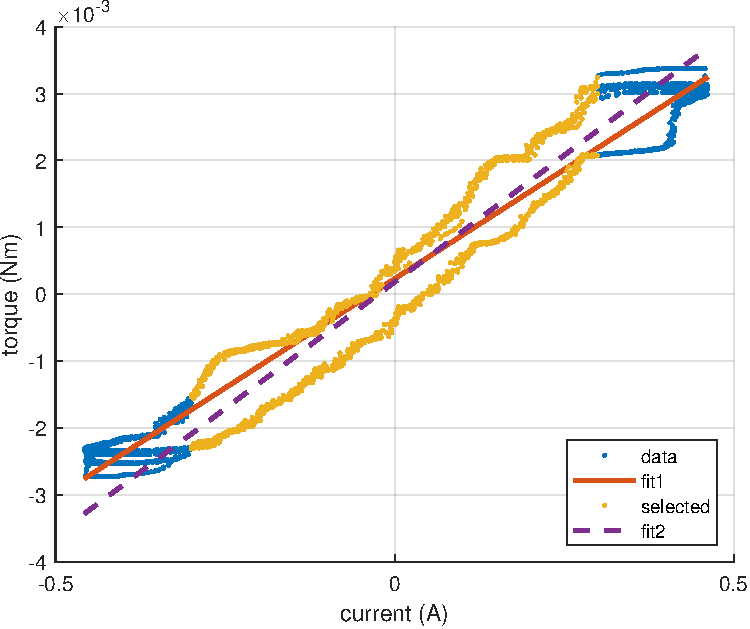
\includegraphics[width=0.75\textwidth]{diagrams/TorqueConstant.pdf}
  \caption{Torque vs commanded current, with linear fits of the entire and partial data set.}
  \label{fig:TorqueConstant}
\end{figure}


\subsection{Friction estimation:}\label{friction}
Since applied torque in Section~\ref{tConstSec} is being estimated from displacement and the frequency is low (which means that inertial and viscous effects are small), the friction shows up as a ``constant'' offset from the ideal torque constant and doesn't affect the slope.
This allows the friction to be seen as half the offset between the data points as the wave maker moves up and down moves down. 
Plotting the torque error using the calculated torque constant against the current gives \figurename~\ref{fig:TorqueError}.
The average offset shows that the static friction is about 0.45\,mNm in this operational envelope.

\begin{figure}[tb]
  \centering
  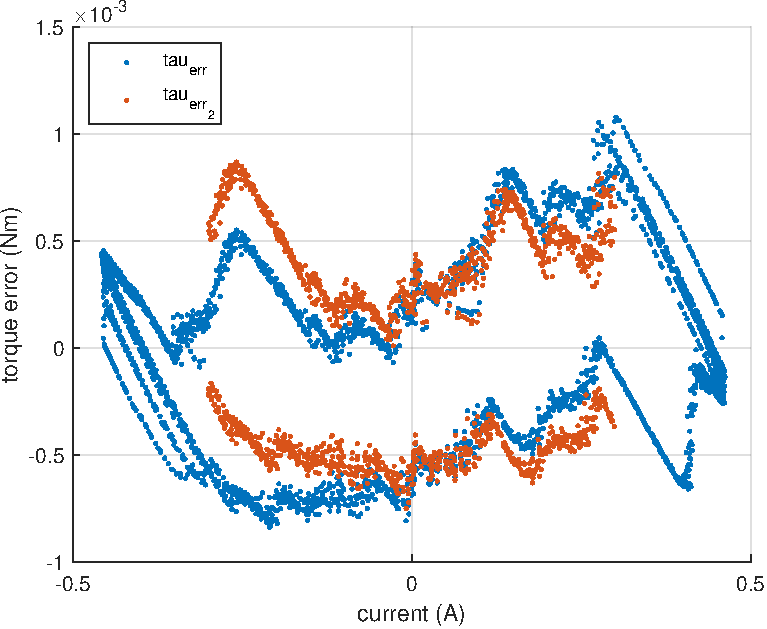
\includegraphics[width=0.75\textwidth]{diagrams/TorqueError.pdf}
  \caption{Motor torque error compared with commanded motor current.}
  \label{fig:TorqueError}
\end{figure}

\subsection{Wave Probes:}	\label{waveprobes}
The readings from the wave probes can be verified by physically attaching the wave probes to the wave maker, which has a very precise encoder that allows for accurate measurement of changes in displacement.
Moving the wave maker with the wave probe attached and comparing the displacement data from both of them was used to make sure the wave probe was providing accurate readings.

It was found having two wave probes quite close together, roughly 1\,ft apart, was problematic.
Changing the depth of one probe seemed to also adjust the reading of the nearby, stationary probe.
It is believed this is caused by capacitive coupling between the two wave probes.
Known work-arounds are only using one probe, or powering the second probe off during operation.

\subsection{WEC feedback control}
The proportional derivative\,(PD) controller functions on the following formula:
%
\begin{equation}  \label{pdctrleq}
  \tau = k_p \cdot p + -k_d \cdot v
\end{equation}
%
Here, $\tau$ is the calculated torque, $k_p$ is the user defined proportional gain, $p$ is the position in meters, $k_d$ is the user defined derivative gain, and $v$ is the velocity, in meters per second, calculated by the change in position over the last 10 milliseconds. 
The torque applied by the motor is thus the combined effect of a spring and damper, with the proportional gain $k_p$ adjusting the strength of the spring, and the derivative gain $k_d$ adjusting the strength of the damper.
Unlike a typical physical spring, this ``spring'' can both push device towards center, or push it away, depending on the sign of the gain.
A positive $k_p$ will act as a destabilizing force, whereas a negative $k_p$ will center the WEC to the waterline, similarly to a physical spring.

The calculation of (\ref{pdctrleq}) is done on the Arduino Due micro-controller responsible for controlling the WEC, which commands an output torque through PWM to the WEC motor controller.
The position and velocity are determined with an encoder, while the $k_p$ and $k_d$ inputs are set by the user in the GUI, which the Arduino receives through USB serial.
By logging the inputs and output of the control system through a range of user inputs, its performance can be verified.
Control loop response times to be less than 33\,ms, as the data logging control loop runs at 30\,Hz and shows a delay of one sample or less.

\figurename~\ref{fig:TorqueCommanded} shows the performance of the controller during typical operation. 
The commanded torque was calculated as per \eqref{pdctrleq}, while the measured torque was taken from an analog output on the WEC motor controller that measures current, then multiplying it by the known torque constant (see Section~\ref{tConstSec}).
This shows us how the PD control algorithm and motor controller react to our given inputs.
As the linearity of the plot shows, the measured output torque closely matches the expected torque.
The standard deviation of the torque during user testing was $3.82 \times 10^{-4}$\,Nm.

\begin{figure}[tb]
  \centering
  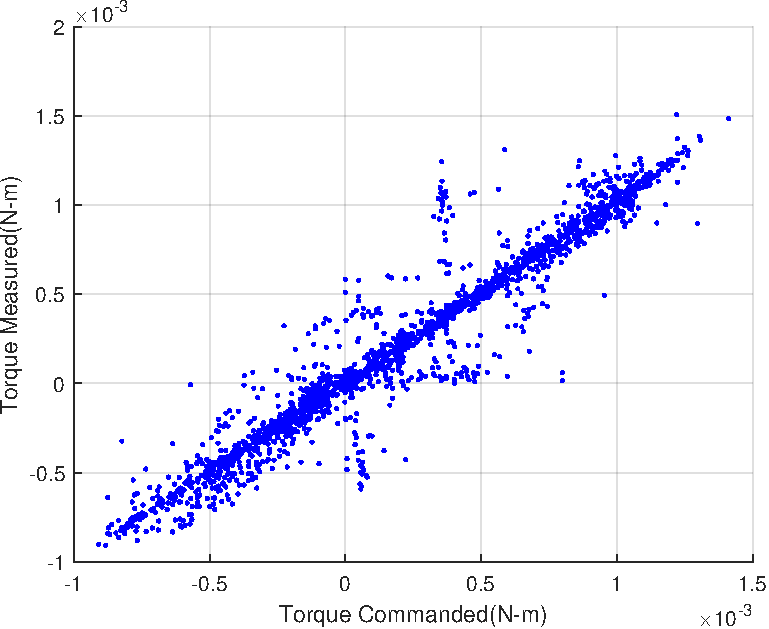
\includegraphics[width=0.75\textwidth]{diagrams/TorqueCommanded.pdf}
  \caption{Comparison of measured and commanded motor torque.}
  \label{fig:TorqueCommanded}
\end{figure}

There is a theoretical possibility to experience saturation near the limits of our torque output.
This is the result of a protection written into the WEC motor controller, and can be adjusted by what is referred to as the ``Thermal Time Constant".
When commanded to apply a torque over what the controller deems as safe, the motor controller will apply this torque for only some time before saturating at the maximum nominal torque.
This was observed targeted testing, occurring around $3.5\times 10^{-3}$\,Nm, but not during any user tests, as the commanded torque was never that high.
If it were to become an issue, the the range of possible $k_p$ and $k_d$ commands and torque jog commands could be limited within the GUI to avoid any saturation triggers.

While fitting closely, there is still error present in this control loop. 
\figurename~\ref{fig:ErrorHistogram} shows a histogram of the torque error, calculated by subtracting the measured torque ($\tau_m$) from the commanded torque ($\tau_c$).
%
\begin{equation}
	\tau_e = \tau_c - \tau_m
	\label{eq:torque_error}
\end{equation}
%
In these particular user tests, the RMS error was $9.84 \times 10^{-5}$\,Nm.
For context, the standard deviation of the torque measurement was $3.82\times 10^{-4}$\,Nm.

\begin{figure}[tb]
  \centering
  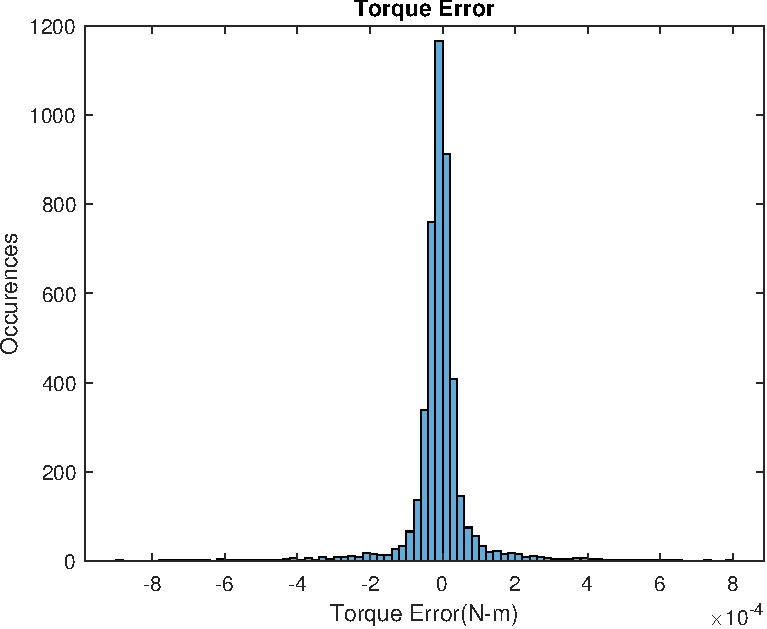
\includegraphics[width=0.75\textwidth]{diagrams/ErrorHistogram.pdf}
  \caption{Histogram of motor torque error per \eqref{eq:torque_error}.}
  \label{fig:ErrorHistogram}
\end{figure}

Part of what has to be considered with this error is noise in the analog signal that is used to read amperage and calculate measured torque.
To characterize this, zero torque can be commanded, and then the measurement analyzed.  
For simplified data collection, user testing data sets were truncated to only sections where the commanded torque was zero.
\figurename~\ref{fig:NoiseHistogram} shows a histogram of the torque when a zero command is sent.
It can be easily seen that there is a slight positive offset in the noise, which is assumed to come from inaccuracy in the analog reporting on the motor controller, or the analog reading on the Arduino Due.
This offset varies from test to test, and can be negative.
Using this method of analyzing only data points where the torque command is zero over multiple tests gives a noise band of about $8 \times 10^{-5}$\,Nm, where 90\% of samples lie between $\pm 4 \times 10^{-5}$\,Nm.
Taken together with the torque error results shown in \figurename~\ref{fig:ErrorHistogram}, this indicates that the system is generally performing close to the limits of the components in terms of repeatability.

\begin{figure}[tb]
  \centering
  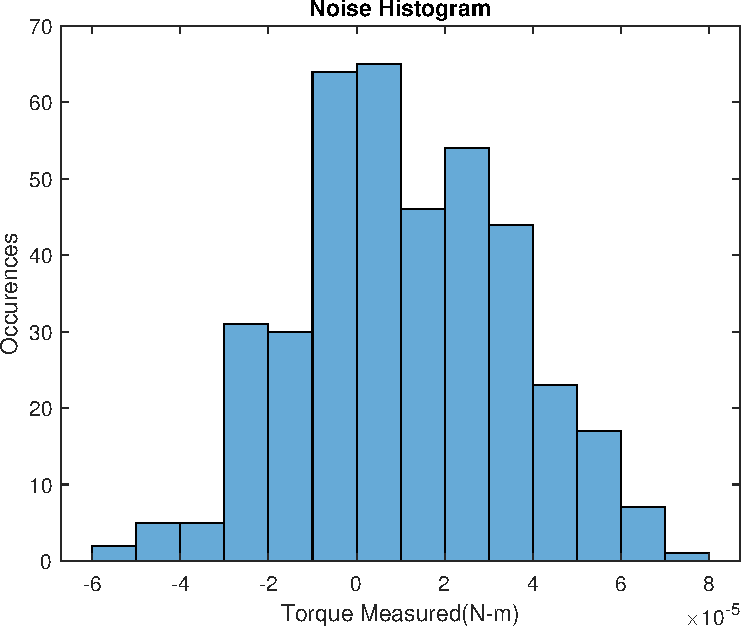
\includegraphics[width=0.75\textwidth]{diagrams/NoiseHistogram.pdf}
  \caption{Histogram of motor torque noise (torque error when commanding zero torque).}
  \label{fig:NoiseHistogram}
\end{figure}

\section{Conclusions}
The SIWEED project was developed to communicate important aspects of WEC design, performance and control while adhering to the open source philosophy. 
This paper provides the resources necessary to understand and even reproduce the SIWEED, while demonstrating the viability of the system. 
With this information in hand, the owners and operators of the SIWEED are now empowered to educate others about wave energy, and any interested parties are enabled to recreate this project.

Should others wish to improve the SIWEED design in future work, the wave probes module would be an excellent area for additional future work.
Because of what was believed to be capacitive coupling as described in Section~\ref{waveprobes}, and limited sensor resolution, the produced waves were never fully characterized to the user.
Communication of wave speed and a more precise wave height measurement in the GUI could prove beneficial to the user. 

%%%%%%%%%%%%%%%%%%%%%%%%%%%%%%%%%%%%%%%%%%
\authorcontributions{Conceptualization, R.G.C., and G.B.; methodology, R.G.C, G.B., S.J.S, A.G.M and D.D.F.; investigation, N.R., D.H., A.G.M., K.D. and A.F.; writing, N.R., A.G.M and R.G.C; project administration, R.G.C; funding acquisition, R.G.C. All authors have read and agreed to the published version of the manuscript.}

\funding{This project was supported by the US Department of Energy's Water Power Technologies Office.}

\dataavailability{This project has been documented through a GitHub repository: \url{https://doi.org/10.5281/zenodo.7502670}.} 

\acknowledgments{
Francisco Colorbio, John Quinlan, and Sean Pluemer worked on an earlier version of the SIWEED project on which this current version was based.
Sandia National Laboratories is a multi-mission laboratory managed and operated by National Technology and Engineering Solutions of Sandia, LLC., a wholly owned subsidiary of Honeywell International, Inc., for the U.S. Department of Energy's National Nuclear Security Administration under contract DE-NA0003525.
This paper describes objective technical results and analysis.
Any subjective views or opinions that might be expressed in the paper do not necessarily represent the views of the U.S. Department of Energy or the United States Government.
}

\conflictsofinterest{The authors declare no conflicts of interest.} 

%%%%%%%%%%%%%%%%%%%%%%%%%%%%%%%%%%%%%%%%%%
%% Optional

%% Only for journal Encyclopedia
%\entrylink{The Link to this entry published on the encyclopedia platform.}

\abbreviations{Abbreviations}{
The following abbreviations are used in this manuscript:\\

\noindent 
\begin{tabular}{@{}ll}
SIWEED & Sandia Interactive Wave Energy Education Display\\
WEC & wave energy converter\\
GUI & graphic user interface\\
JONSWAP & Joint North Sea Wave Project\\
CAD & computer aided design\\
PWM & pulse width modulation\\
SPI & serial peripheral interface\\
SID & system identification\\
IDE & integrated development environment\\
USB & universal serial bus\\
PD & proportional-derivative\\
RMS & root-mean-square\\
LED & light emitting diode
\end{tabular}
}

% %%%%%%%%%%%%%%%%%%%%%%%%%%%%%%%%%%%%%%%%%%
% %% Optional
% \appendixtitles{no} % Leave argument "no" if all appendix headings stay EMPTY (then no dot is printed after "Appendix A"). If the appendix sections contain a heading then change the argument to "yes".
\appendixstart
\appendix
\section[\appendixname~\thesection]{Detailed design documents}
Detailed electrical schematics are provided in \figurename~\ref{fig:siweed_electronics}-\ref{fig:siweed_electronics_aux_subsystems}.
A detailed bill of materials is provided in Table~\ref{tab:bom}.

\begin{landscape}
\begin{figure}[tb]
	\centering
	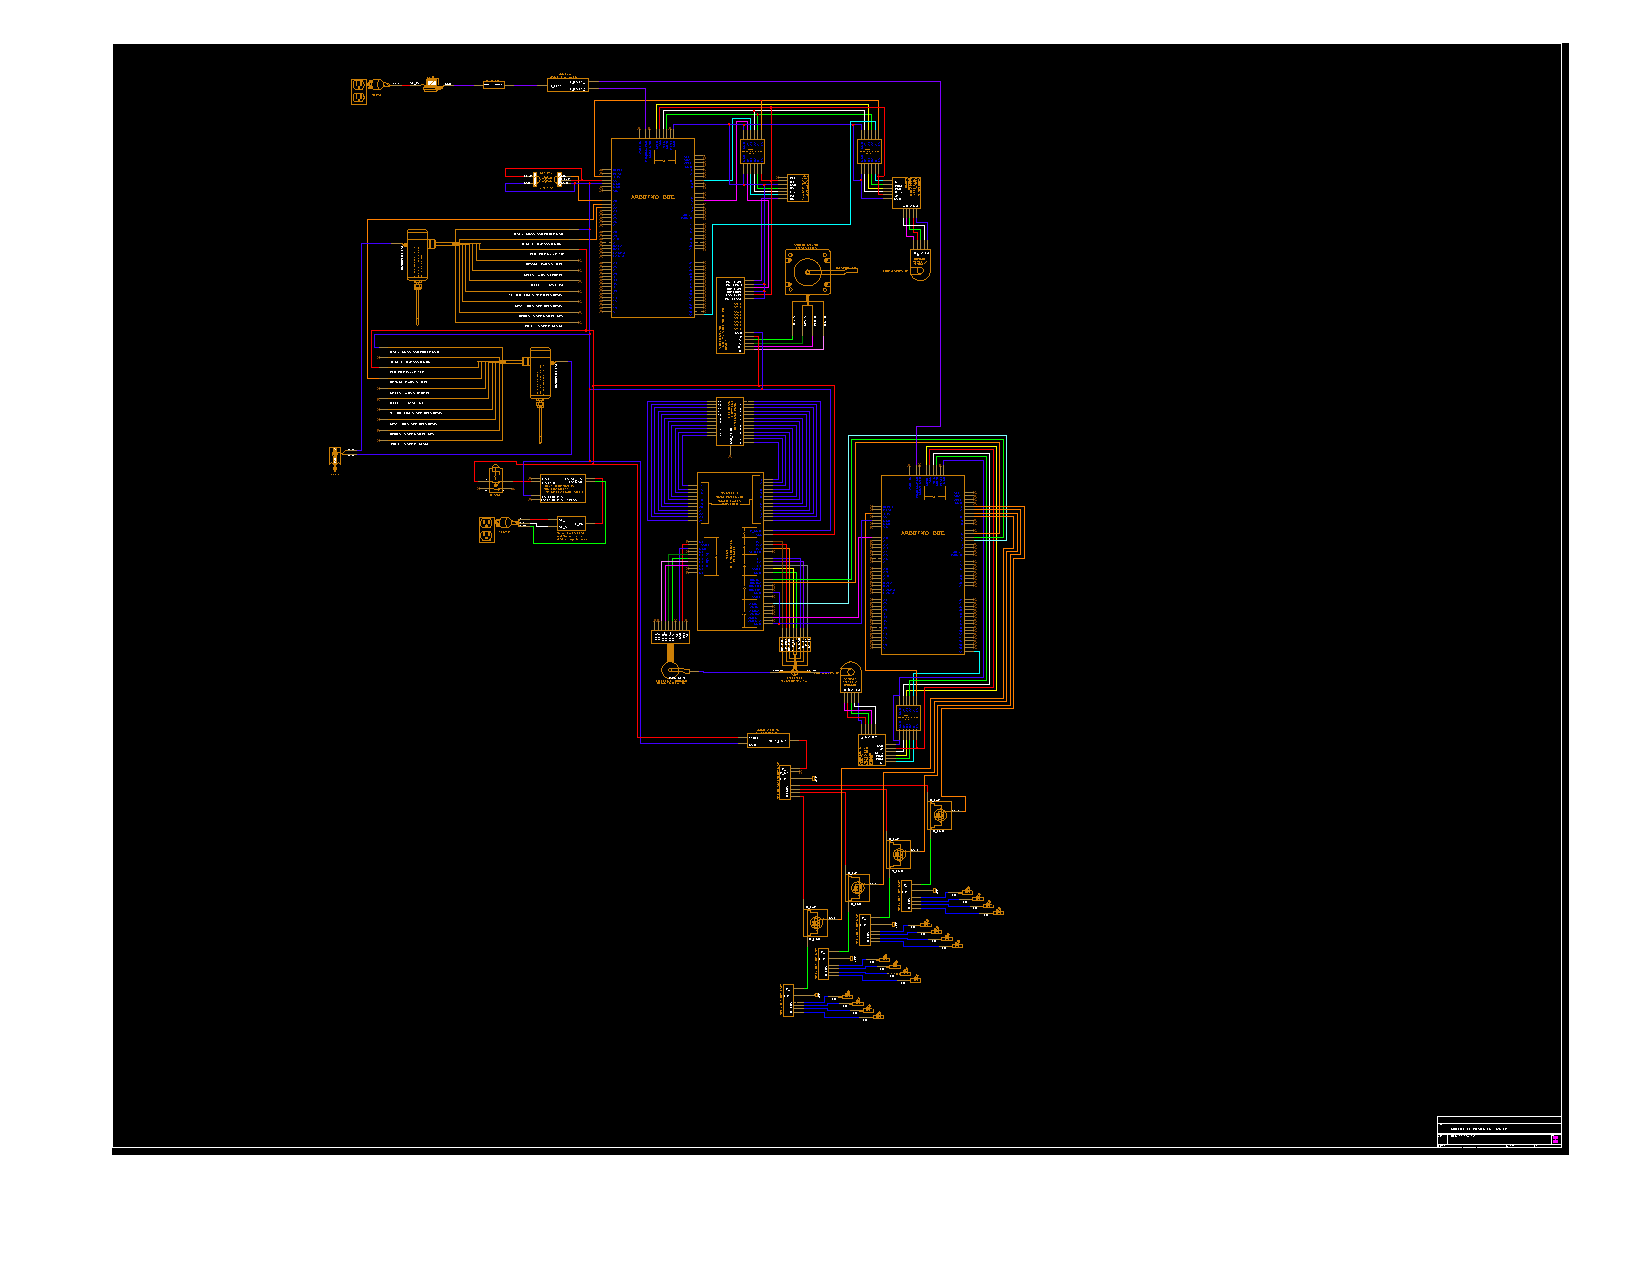
\includegraphics[height=0.95\textwidth, width=\linewidth]{diagrams/SIWEED_ElecDrawings_and_UpdatedBOM/PDFs/siweed_electronics.pdf}
	\caption{Overall electronics schematic.}
	\label{fig:siweed_electronics}
\end{figure}
\end{landscape}

\begin{landscape}
\begin{figure}[tb]
	\centering
	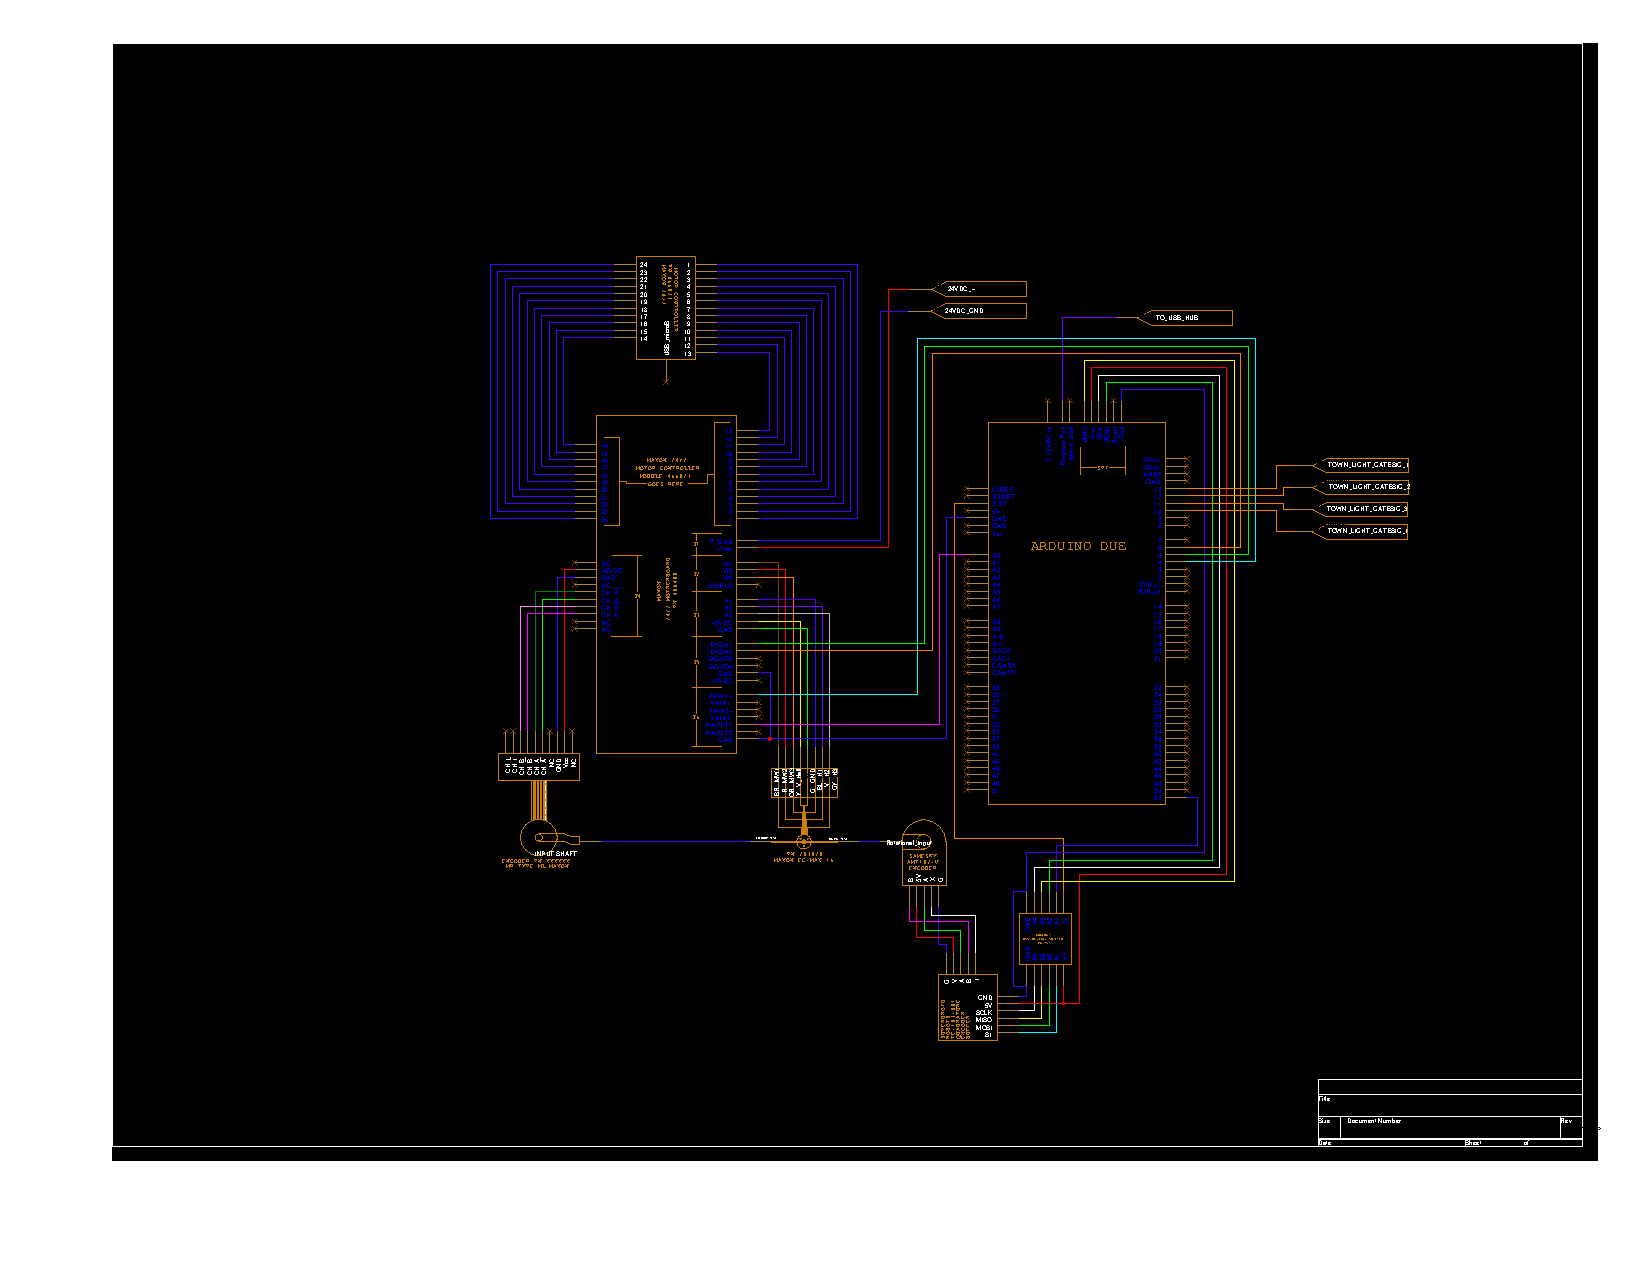
\includegraphics[height=0.95\textwidth, width=\linewidth]{diagrams/SIWEED_ElecDrawings_and_UpdatedBOM/PDFs/siweed_electronics_wec_only.pdf}
	\caption{WEC electronics schematic.}
	\label{fig:siweed_electronics_wec_only}
\end{figure}
\end{landscape}

\begin{landscape}
\begin{figure}[tb]
	\centering
	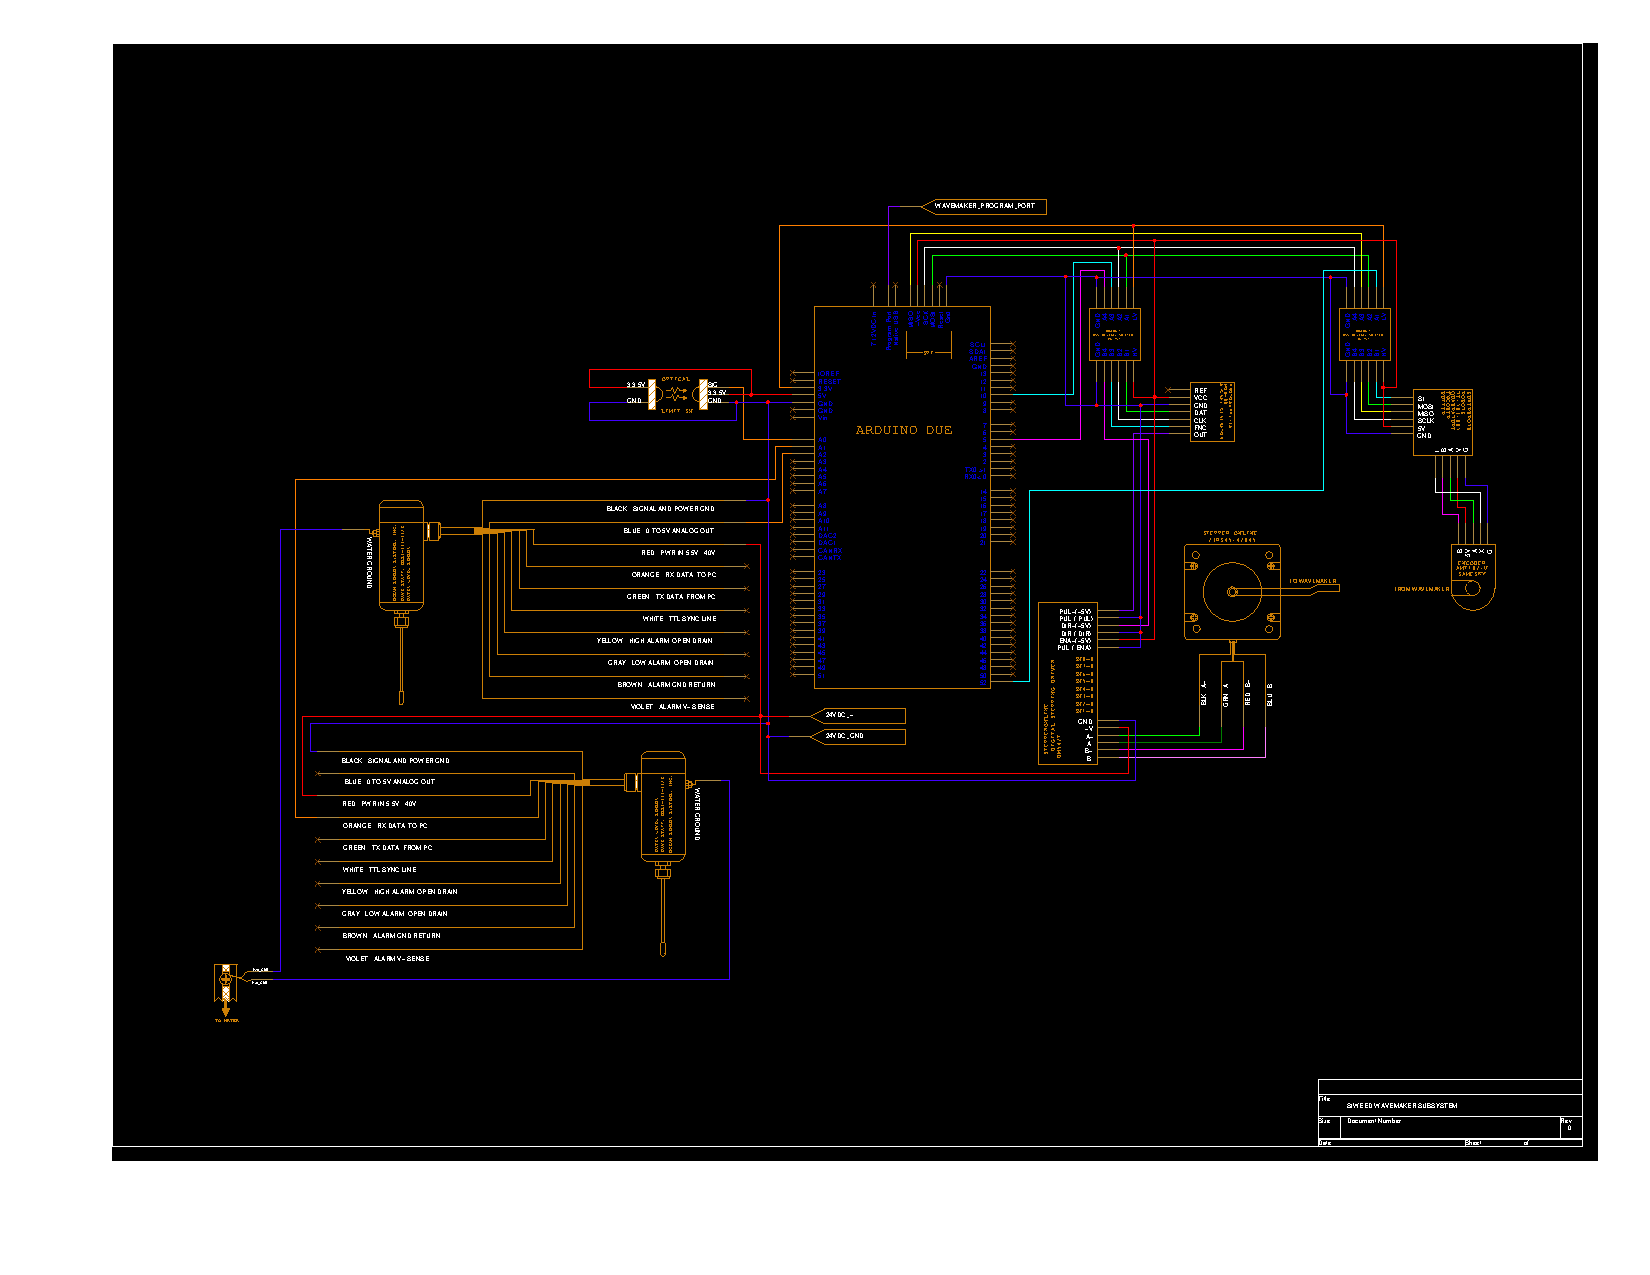
\includegraphics[height=0.95\textwidth, width=\linewidth]{diagrams/SIWEED_ElecDrawings_and_UpdatedBOM/PDFs/siweed_electronics_wavemaker_only.pdf}
	\caption{Wave maker electronics schematic.}
	\label{fig:siweed_electronics_wavemaker_only}
\end{figure}
\end{landscape}

\begin{landscape}
\begin{figure}[tb]
	\centering
	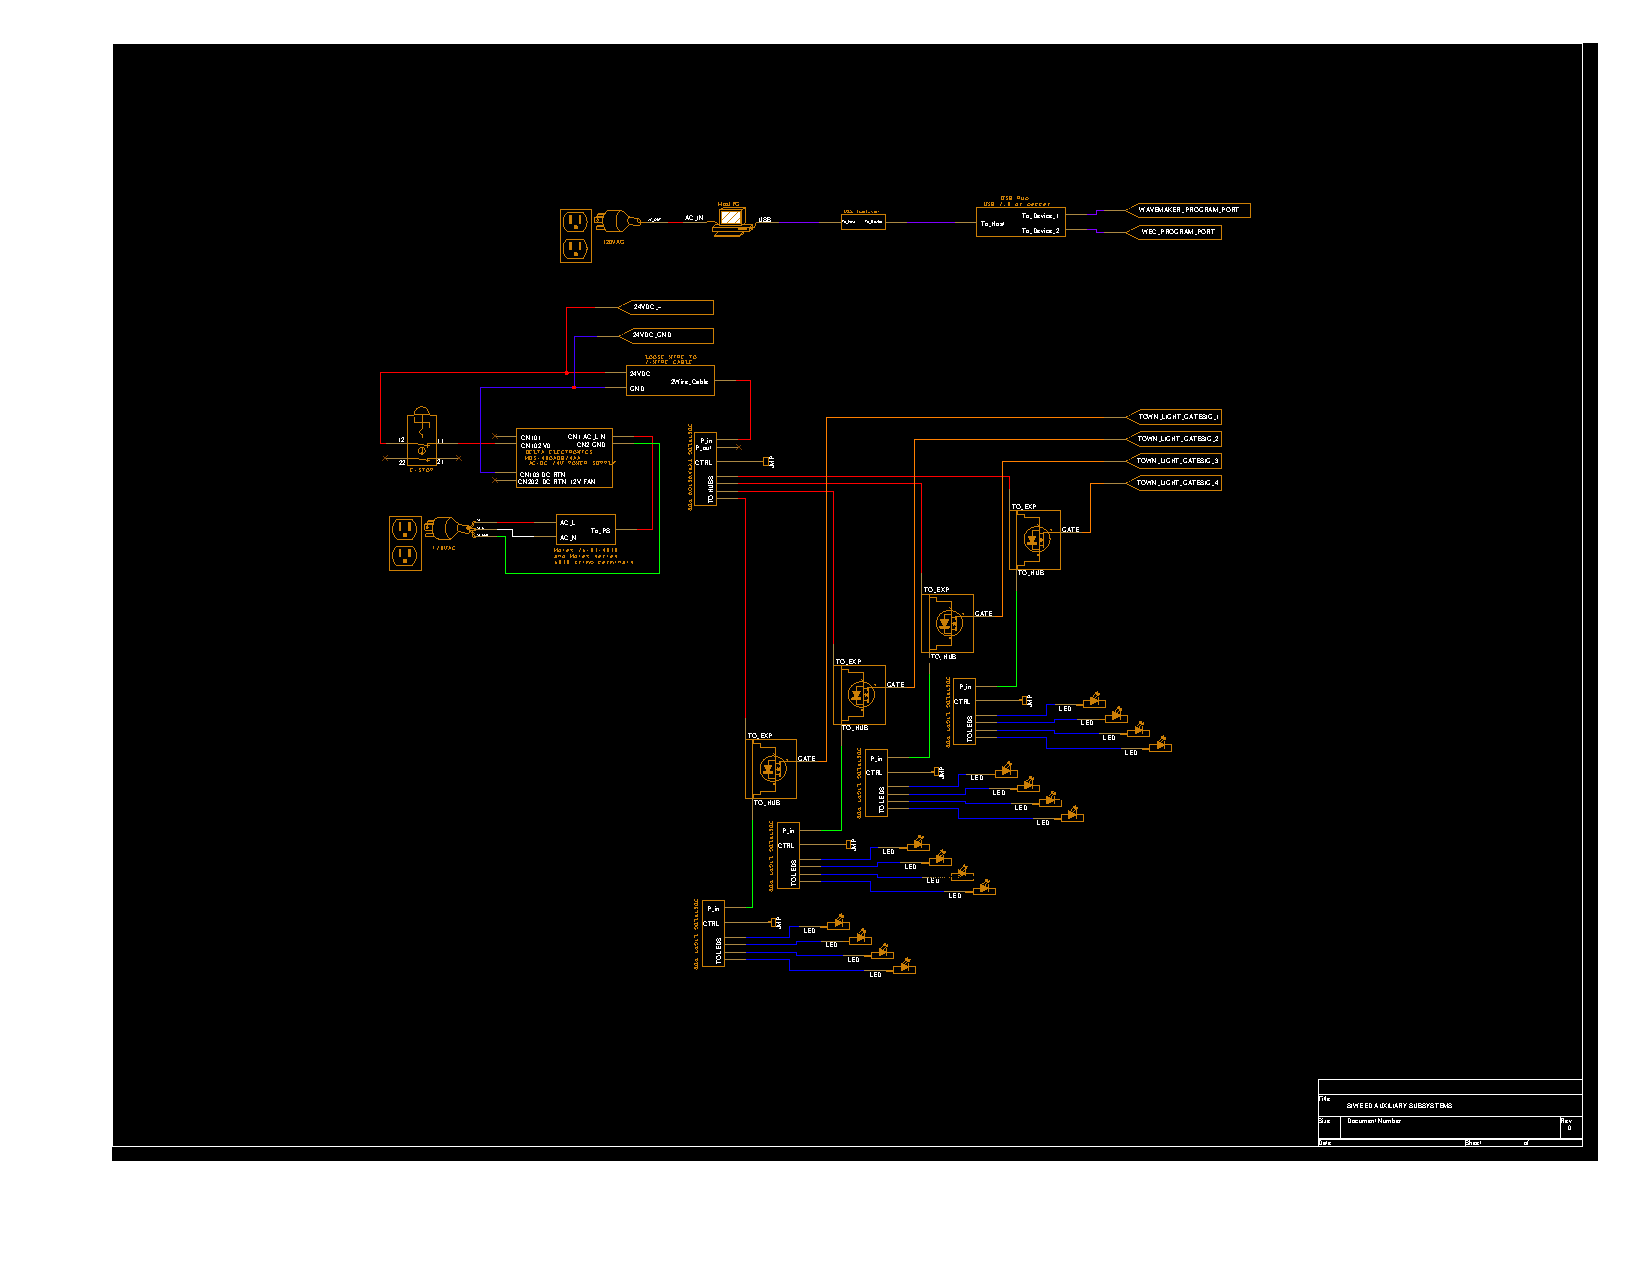
\includegraphics[height=0.95\textwidth, width=\linewidth]{diagrams/SIWEED_ElecDrawings_and_UpdatedBOM/PDFs/siweed_electronics_aux_subsystems.pdf}
	\caption{Wave maker electronics schematic.}
	\label{fig:siweed_electronics_aux_subsystems}
\end{figure}
\end{landscape}



\DTLloaddb{data}{BOM.csv}

\begin{landscape}
\begingroup
\footnotesize
\renewcommand{\dtldisplaystarttab}{\hline}%
\renewcommand\dtldisplayafterhead{\hline}%
\renewcommand\dtldisplaystartrow{\hline}%

\DTLdisplaylongdb[caption=Bill of materials., contcaption=Bill of materials (continued)., label=tab:bom]{data}
\end{landscape}
\endgroup



% \subsection[\appendixname~\thesubsection]{}
% The appendix is an optional section that can contain details and data supplemental to the main text---for example, explanations of experimental details that would disrupt the flow of the main text but nonetheless remain crucial to understanding and reproducing the research shown; figures of replicates for experiments of which representative data are shown in the main text can be added here if brief, or as Supplementary Data. Mathematical proofs of results not central to the paper can be added as an appendix.

% \begin{table}[H] 
% \caption{This is a table caption.\label{tab5}}
% \newcolumntype{C}{>{\centering\arraybackslash}X}
% \begin{tabularx}{\textwidth}{CCC}
% \toprule
% \textbf{Title 1}	& \textbf{Title 2}	& \textbf{Title 3}\\
% \midrule
% Entry 1		& Data			& Data\\
% Entry 2		& Data			& Data\\
% \bottomrule
% \end{tabularx}
% \end{table}

% \section[\appendixname~\thesection]{}
% All appendix sections must be cited in the main text. In the appendices, Figures, Tables, etc. should be labeled, starting with ``A''---e.g., Figure A1, Figure A2, etc.

%%%%%%%%%%%%%%%%%%%%%%%%%%%%%%%%%%%%%%%%%%
\begin{adjustwidth}{-\extralength}{0cm}
%\printendnotes[custom] % Un-comment to print a list of endnotes

\reftitle{References}

\bibliography{siweedPaper}

\PublishersNote{}
\end{adjustwidth}
\end{document}

